\appendix{

\subsection{Advantages of Using an Action Filter}\label{appendix:lpf}
We used a Low Pass Filter (LPF) after the policy output, acting as an action filter. The LPF used in this work is a Butterworth low pass filter with a cut-off frequency of 4 Hz. LPF has been widely applied in control engineering including model-based optimal control methods~\citep{gong2022zero} and model-free RL methods~\citep{peng2020learning,li2021reinforcement,smith2022legged,escontrela2022adversarial} for legged locomotion. 
LPF can further smooth out the action from the RL-based policy, which further complements the smoothing rewards listed in Table~\ref{tab:reward}.
We conducted an ablation study by training a jumping-in-place policy (single-task training) \emph{without} LPF, which still results in jumping but with worse learning performance (converged return) due to the resulting jittering motion, as shown in Fig.~\ref{subfig:lpf_benchmark}. 
If we take out the LPF, we will need to increasing the weight on the smoothing term to highlight the importance of the smoothness of the entire motion. However, if the smoothing term takes too much weight in the entire reward composition, the robot may easily learn a suboptimal behavior by being stationary without exploring dynamic skills such as jumping. Therefore, LPF can help with reducing such reward tuning burden.
Furthermore, since LPF only helps to damp out the high-frequency changes from the action (policy's output), the entire system may still have oscillation (\textit{e.g.}, due to a large joint velocity), having the smoothing reward is still necessary to smooth the entire closed-loop system. These two parts complement each other.


\begin{figure}[!]
\centering
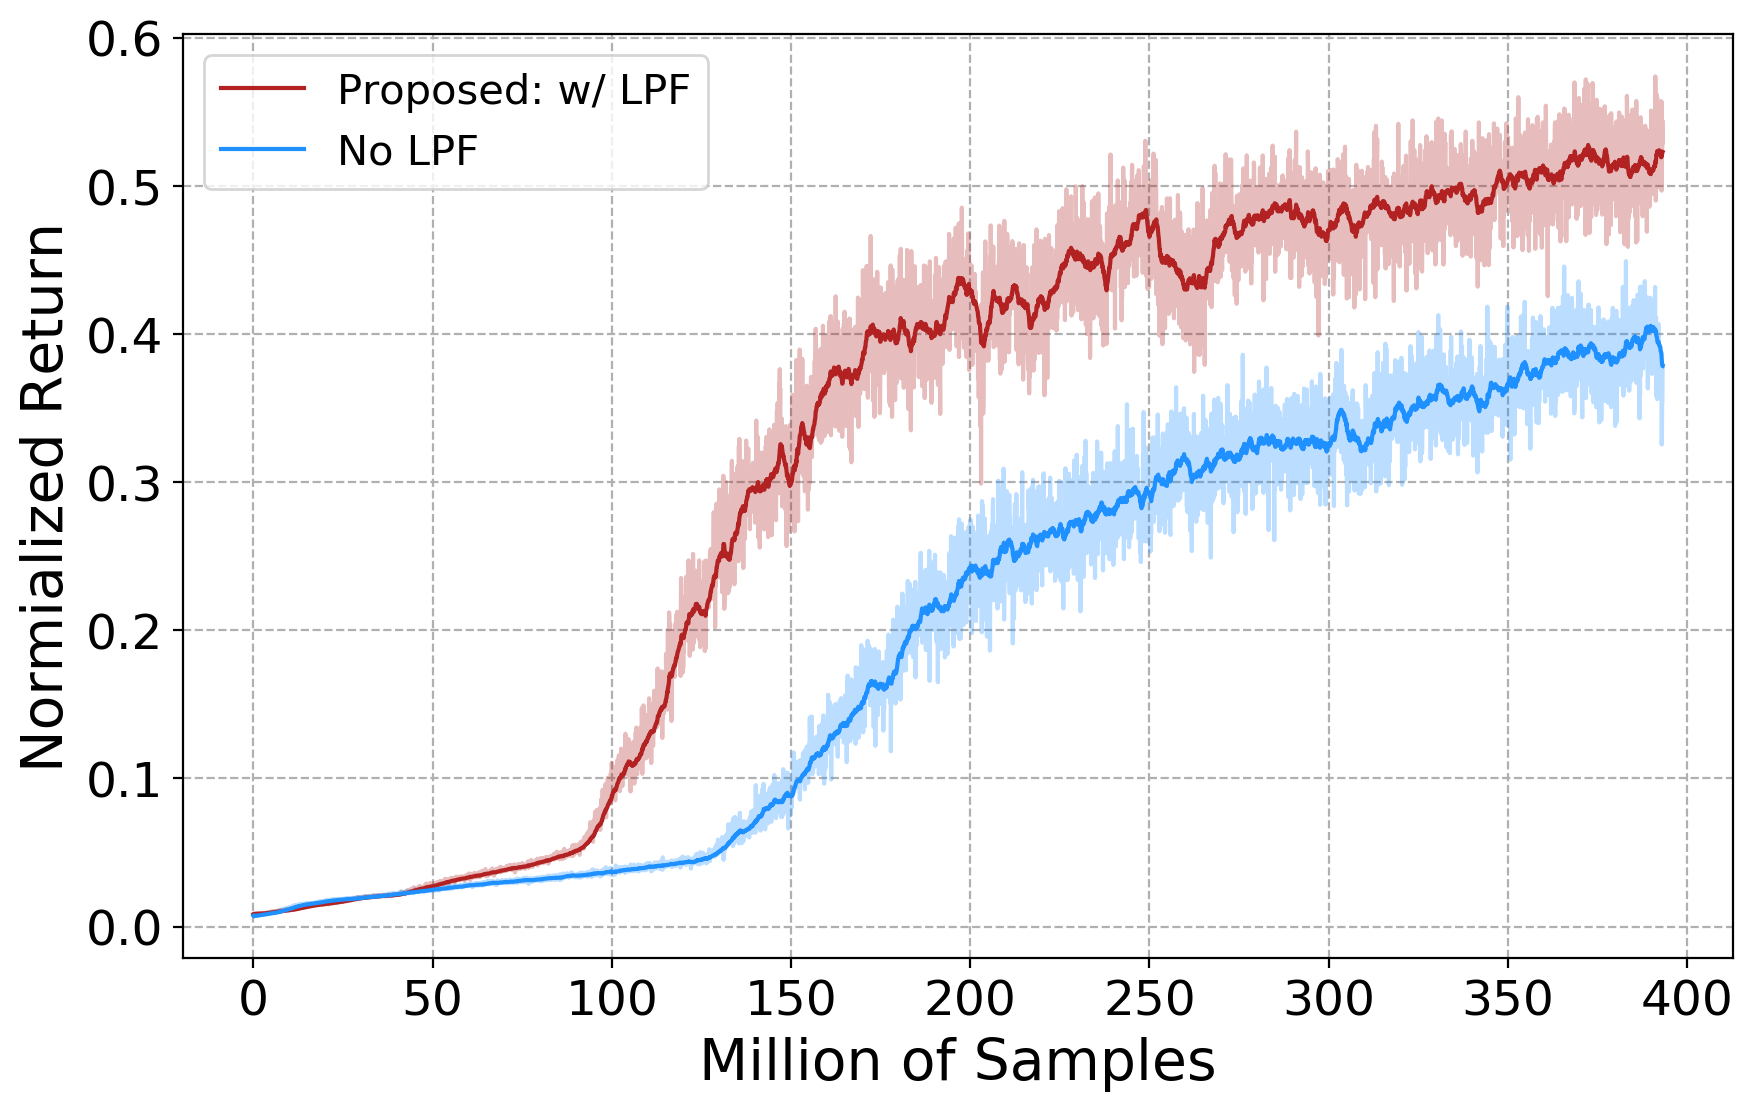
\includegraphics[width=0.75\linewidth]{figures/lpf_benchmark.png}
\caption{Ablation study on the use of Low Pass Filter (LPF) as an action filter for the training of the in-place jumping skill from scratch. Without using the LPF, the training return (blue curve) is much lower than the one using LPF (ours, red curve). These two policies are obtained by using the exact hyperparameters and training settings. The underlying reason is that it is harder for the RL-based policy to damp out high-frequency jittering motion without the use of LPF.}\label{subfig:lpf_benchmark}
\end{figure}


\subsection{Learning to Combine a Standing Skill}\label{appendix:transition_to_stand}
Enabling the robot to learn standing along with other locomotion skills is useful for real-world applications, as it is essential to retrieve the physical robot hardware (while the robot is not moving). 

For the walking skill, after the robot has mastered the diverse walking tasks after the task randomization stage, we added a sub-stage. 
In the episode of this sub-stage of training, a standing skill is commanded after a random timespan of walking, and \emph{will last until the end of episode}. The robot is informed to perform standing by two changes: (1) the reference motion input to the control policy is changed to a nominal standing motion (the preview of reference motion is now a stack of three same standing motor positions), and (2) the reward is formulated to encourage performing stationary standing skill. 
The reward for standing has the same formulation used for training dynamic locomotion skills listed in Table~\ref{tab:reward}, and the weights of smoothing terms, such as motor velocity and change of action, are increased with other terms remaining unchanged.
The increased smoothing weight is to encourage the robot to maintain a stationary standing pose. 
After the robot has acquired the skills of walking, standing, and the transition from an arbitrary state from walking to standing, we can move on to dynamics randomization. 
Starting from this stage, the standing skill will be only introduced in the middle of the training of walking and last for a random finite timespan. In this way, the robot can also learn the transition back from standing to walking.  

For the running skill, the POMDP design for this sub-stage is similar to the one for walking. However, since transiting from fast running to standing is more challenging, we provide an additional reference motion of transition from running to standing, retargeted from human mocap. This could facilitate the training during the transition phase. 
For the jumping skill, since it is an aperiodic skill and the robot is required to maintain a standing pose after landing, we do not need such an additional sub-stage of training.       

This method may also be useful to combine different locomotion skills (like combining all walking, running, and jumping) using one single policy. This could potentially solve the problem of developing multi-skill policy for highly-dynamic legged locomotion control. 
We note this as a possible extension of this work.  



\subsection{Command Range for Different Skills}\label{appendix:command}

\begin{table}[!ht]
\centering
\scriptsize
\caption{Command range for different skills.}
\label{tab:command}
\begin{tabular}{|cc|}
\hline
\multicolumn{1}{|c|}{\textbf{Task Parameters}}          & \textbf{Range}        \\ \hline
\multicolumn{2}{|c|}{\textbf{Walking}}                                          \\ \hline
\multicolumn{1}{|c|}{Sagittal Velocity $\dot{q}^d_x$}   & {[}-1.5, 1.5{]} m/s   \\ \hline
\multicolumn{1}{|c|}{Lateral Velocity $\dot{q}^d_y$}    & {[}-0.6, 0.6{]} m/s   \\ \hline
\multicolumn{1}{|c|}{Turning Velocity $\dot{q}^d_\psi$} & {[}-45, 45{]} deg/s   \\ \hline
\multicolumn{1}{|c|}{Walking Height $q^d_z$}            & {[}0.65, 1.0{]} m     \\ \hline
\multicolumn{2}{|c|}{\textbf{Running}}                                          \\ \hline
\multicolumn{1}{|c|}{Sagittal Velocity $\dot{q}^d_x$}   & {[}2.0, 5.0{]} m/s    \\ \hline
\multicolumn{1}{|c|}{Lateral Velocity $\dot{q}^d_y$}    & {[}-0.75, 0.75{]} m/s \\ \hline
\multicolumn{1}{|c|}{Turning Velocity $\dot{q}^d_\psi$} & {[}-30, 30{]} deg/s   \\ \hline
\multicolumn{2}{|c|}{\textbf{Jumping}}                                          \\ \hline
\multicolumn{1}{|c|}{Sagittal Landing Location $q^d_x$} & {[}-0.5, 1.5{]} m     \\ \hline
\multicolumn{1}{|c|}{Lateral Landing Location $q^d_y$}  & {[}-1.0 1.0{]} m      \\ \hline
\multicolumn{1}{|c|}{Turning Direction at Landing $q^d_\psi$} & {[}-100, 100{]} deg \\ \hline
\multicolumn{1}{|c|}{Change of Elevation $e^d_z$}       & {[}-0.5, 0.5{]} m     \\ \hline
\end{tabular}
\end{table}

The training ranges for the command of three locomotion skills (walking, running, and jumping) developed in this work are detailed in Table ~\ref{tab:command}. 
During a training episode, the given command is drawn uniformly from the listed range.  

\subsection{Hyperparameters Used in Training}\label{appendix:hyperparameters}



\begin{table*}[!]
\scriptsize
\centering
\caption{Number of Training Iterations used for Different Locomotion Skills. Each iteration collects a batch of 65536 samples.}
\label{tab:num_iter}
\begin{tabular}{|ccccc|}
\hline
\multicolumn{5}{|c|}{\textbf{Walking}} \\ \hline
\multicolumn{1}{|c|}{Single-Task} & \multicolumn{1}{c|}{Task Randomization} & \multicolumn{1}{c|}{Combining Standing} & \multicolumn{1}{c|}{Dynamics Randomization} & Added Perturbation Training \\ \hline
\multicolumn{1}{|c|}{6000} & \multicolumn{1}{c|}{8000} & \multicolumn{1}{c|}{2000} & \multicolumn{1}{c|}{8000} & 5000 \\ \hline
\multicolumn{5}{|c|}{\textbf{Running}} \\ \hline
\multicolumn{1}{|c|}{Single-Task} & \multicolumn{1}{c|}{Task Randomization} & \multicolumn{1}{c|}{Combining Standing} & \multicolumn{1}{c|}{Dynamics Randomization} & Added Perturbation Training \\ \hline
\multicolumn{1}{|c|}{6000} & \multicolumn{1}{c|}{18000} & \multicolumn{1}{c|}{5000} & \multicolumn{1}{c|}{15000} & 5000 \\ \hline
\multicolumn{5}{|c|}{\textbf{Jumping}} \\ \hline
\multicolumn{1}{|c|}{Single-Task} & \multicolumn{1}{c|}{Task Randomization} & \multicolumn{1}{c|}{} & \multicolumn{1}{c|}{Dynamics Randomization} &  \\ \hline
\multicolumn{1}{|c|}{6000} & \multicolumn{1}{c|}{12000} & \multicolumn{1}{c|}{} & \multicolumn{1}{c|}{20000} &  \\ \hline
\end{tabular}
\end{table*}
\begin{table}[!]
\scriptsize
\centering
\caption{Hyperparameters used in PPO Training. These are consistent among different locomotion skills.}
\label{tab:hyperparam_ppo}
\begin{tabular}{|l|l|}
\hline
\textbf{Hyperparameter} & \textbf{Value} \\ \hline
PPO iteration batch size & 65536 \\ \hline
PPO clip rate & 0.2 \\ \hline
Optimization step size (both actor and critic) & $1e^{-4}$ \\ \hline
Optimization batch size & 8192 \\ \hline
Optimization epochs & 2 \\ \hline
Discount factor ($\gamma$) & 0.98 \\ \hline
GAE smoothing factor ($\lambda$) & 0.95 \\ \hline
\end{tabular}
\end{table}

The number of training (PPO) iterations used to develop different locomotion skills is detailed in Table~\ref{tab:num_iter}.
Furthermore, the hyperparameters of PPO are reported in Table~\ref{tab:hyperparam_ppo}, and they are consistent over different locomotion skills. 




\subsection{Comparison of Use of Different History Lengths}\label{appendix:history_length}

\begin{figure}[ht]
\centering
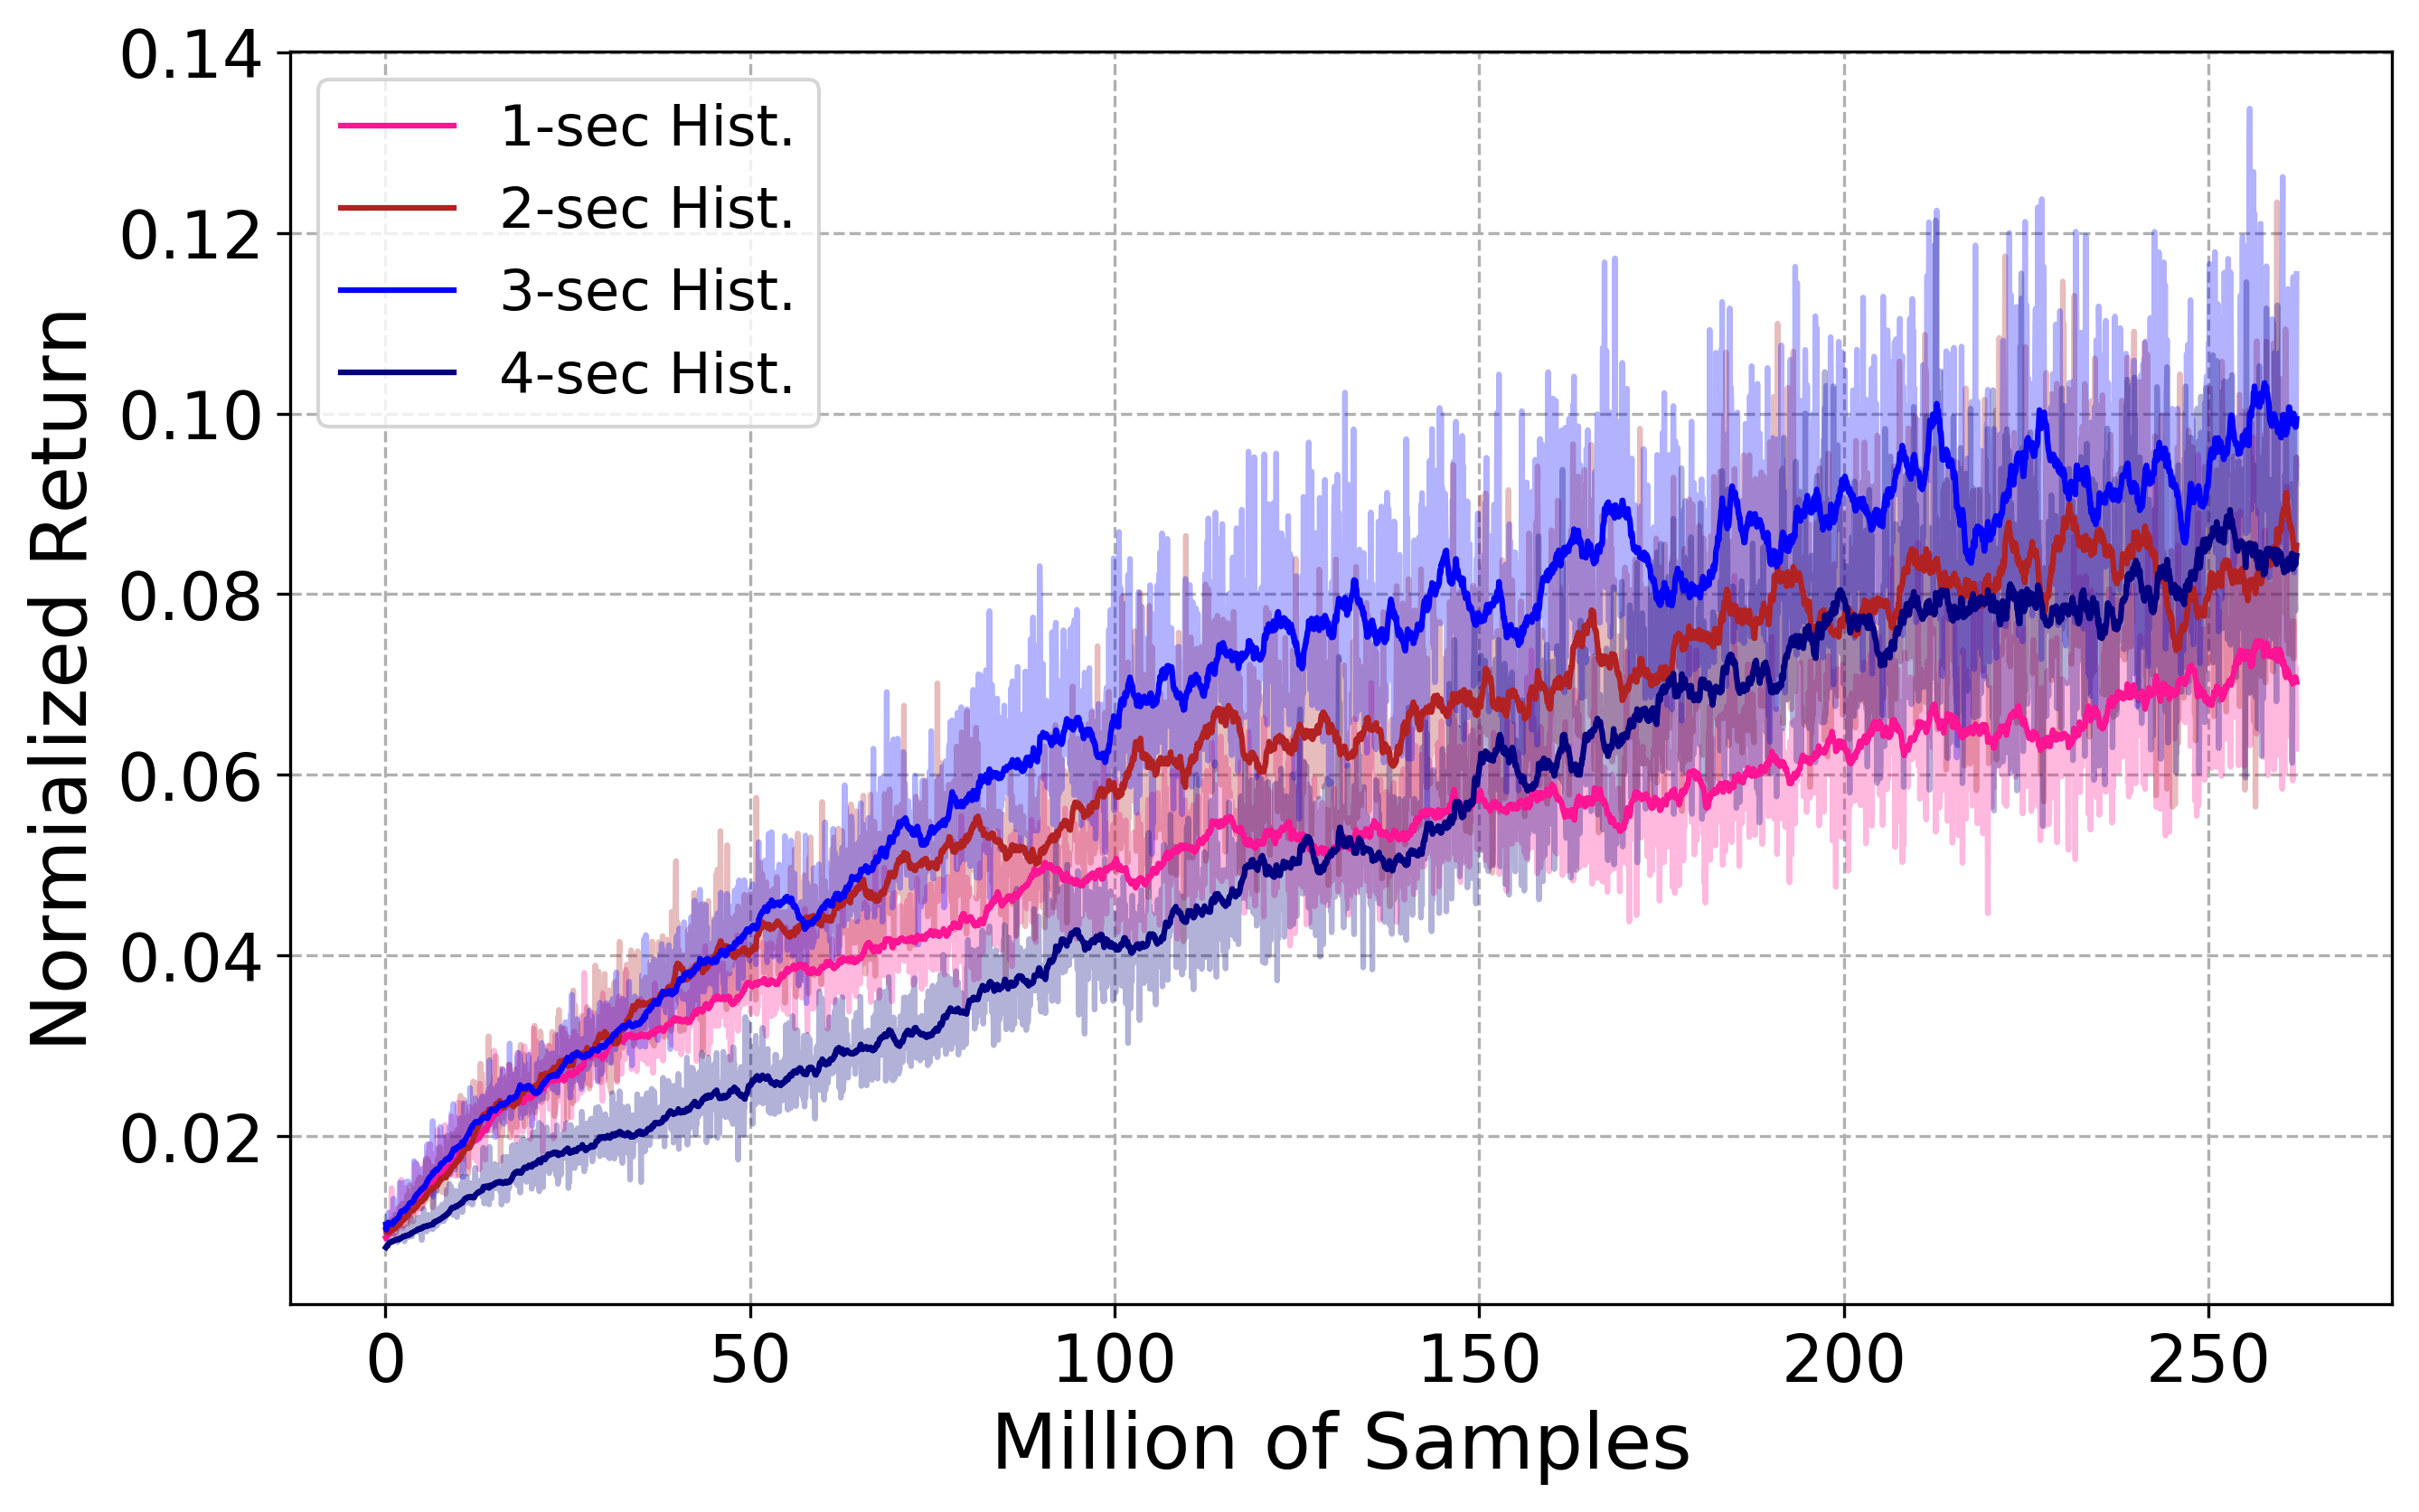
\includegraphics[width=0.75\linewidth]{figures/single_dynrand_hist_compare_logs_run.png}
\caption{Learning performance using different lengths of the robot's I/O history when training a single-task running policy with dynamics randomization. All of these policies used the proposed dual-history-based policy. When increasing the explicit length of robot history from 1 second (pink curve), 2 seconds (red curve, as used in this work), and 3 seconds (blue curve), we observe an increase in learning performance. However, if we keep increasing the history length, such as to 4 seconds (dark blue curve), the improvement of the learning performance may get saturated.}
\label{fig:hist_compare}
\end{figure}



\begin{figure}[ht]
\centering
\begin{subfigure}{0.475\linewidth}
  \centering
  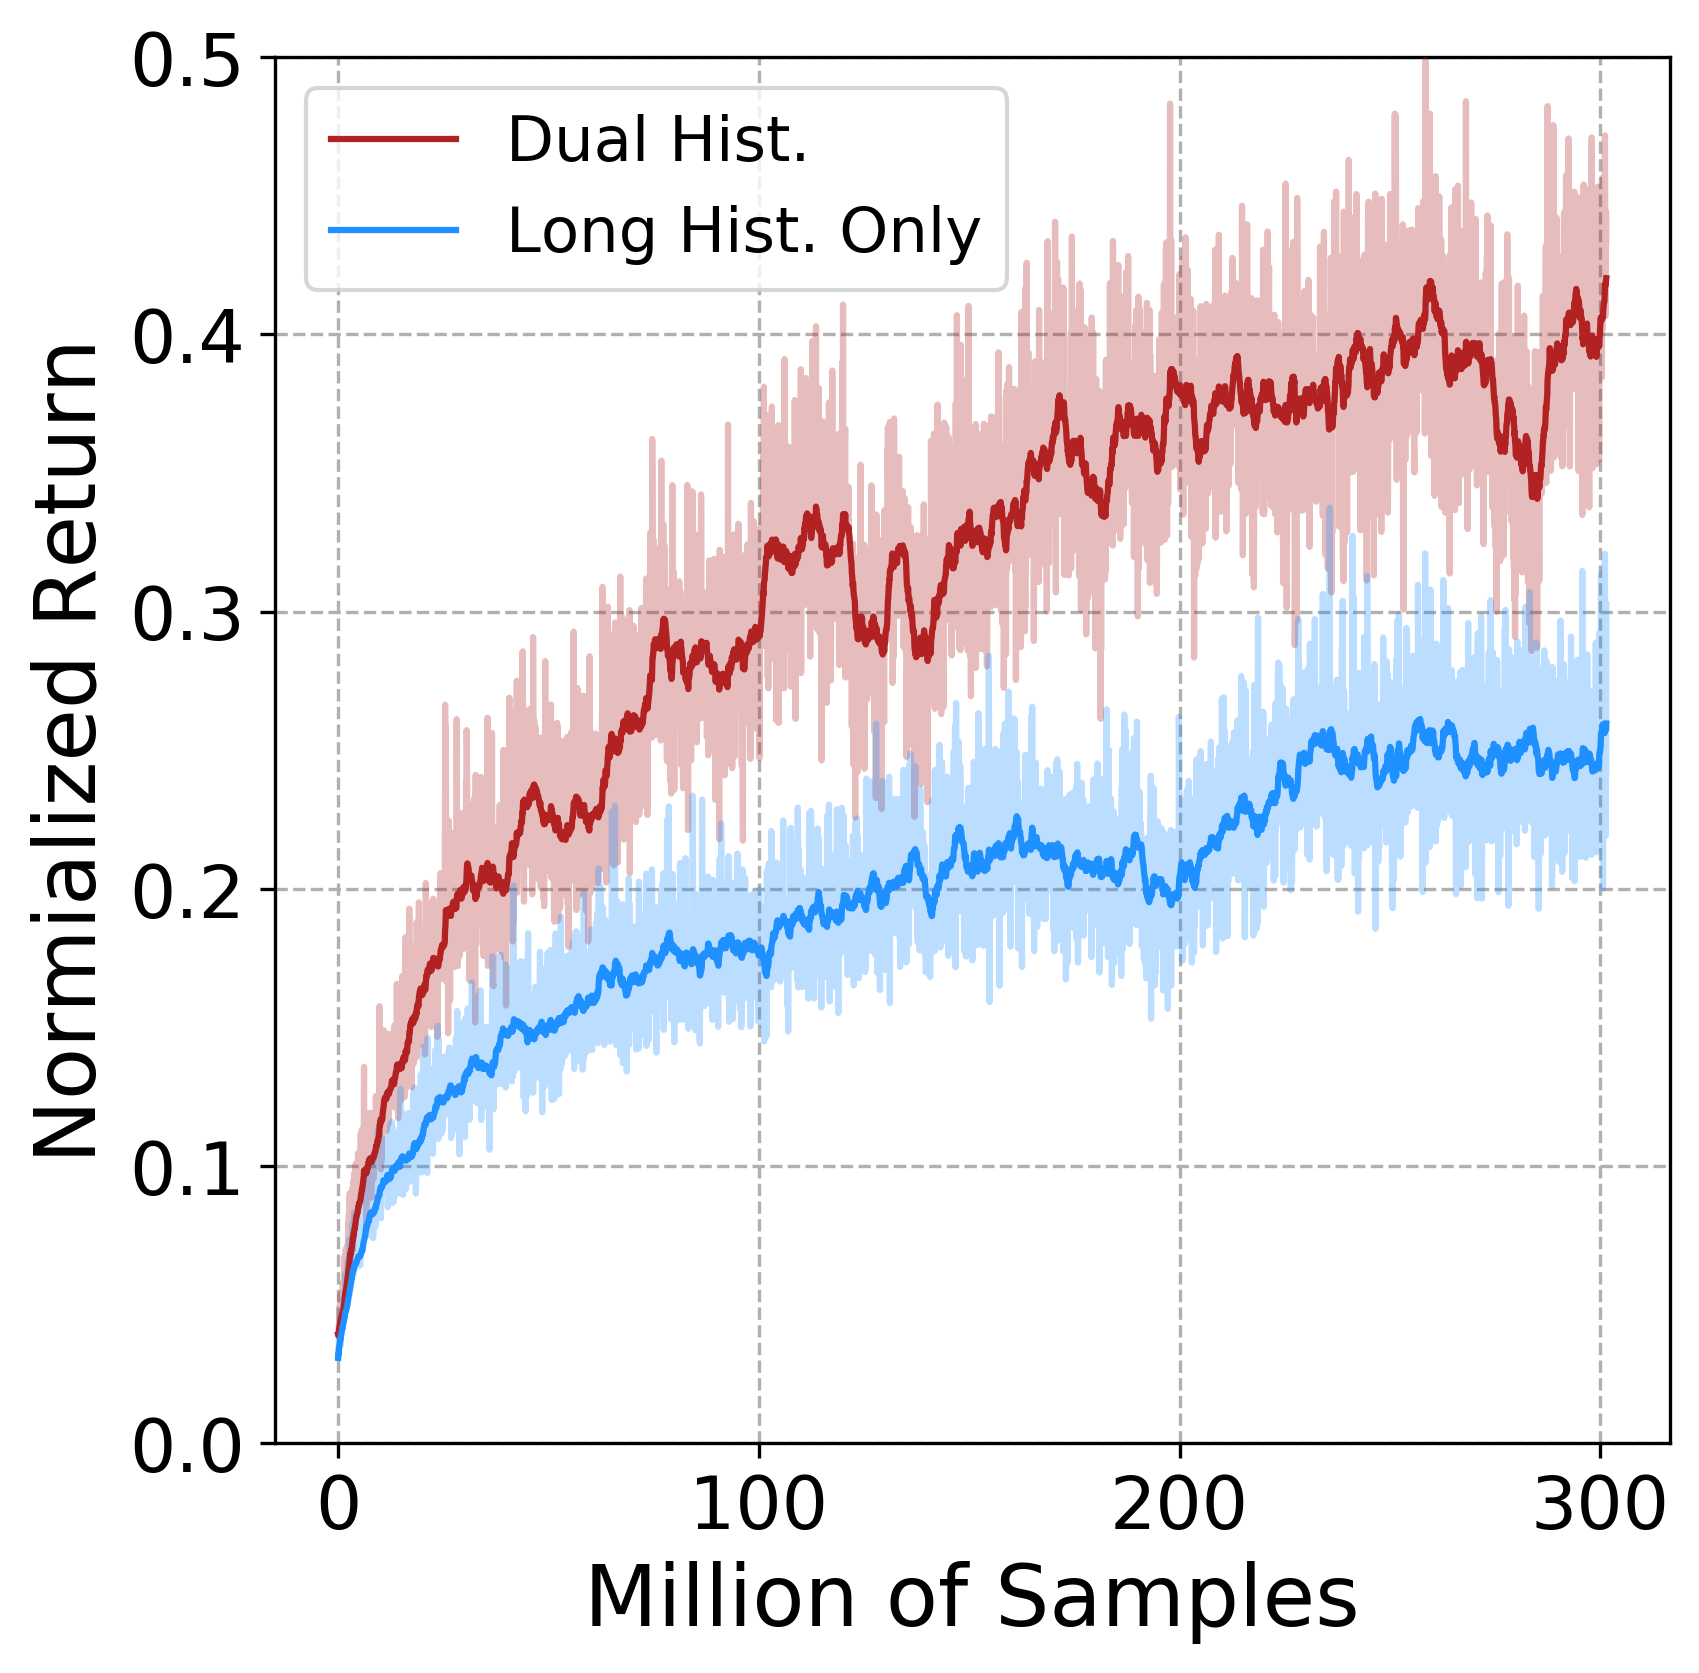
\includegraphics[width=\linewidth]{figures/single_dynrand_tcn_same_compare_logs_v2.png}
  \caption{TCN with dual history approach (Dual Hist.) and the TCN only (Long Hist. Only).}
  \label{subfig:tcn_compare}
\end{subfigure}
\begin{subfigure}{0.475\linewidth}
  \centering
  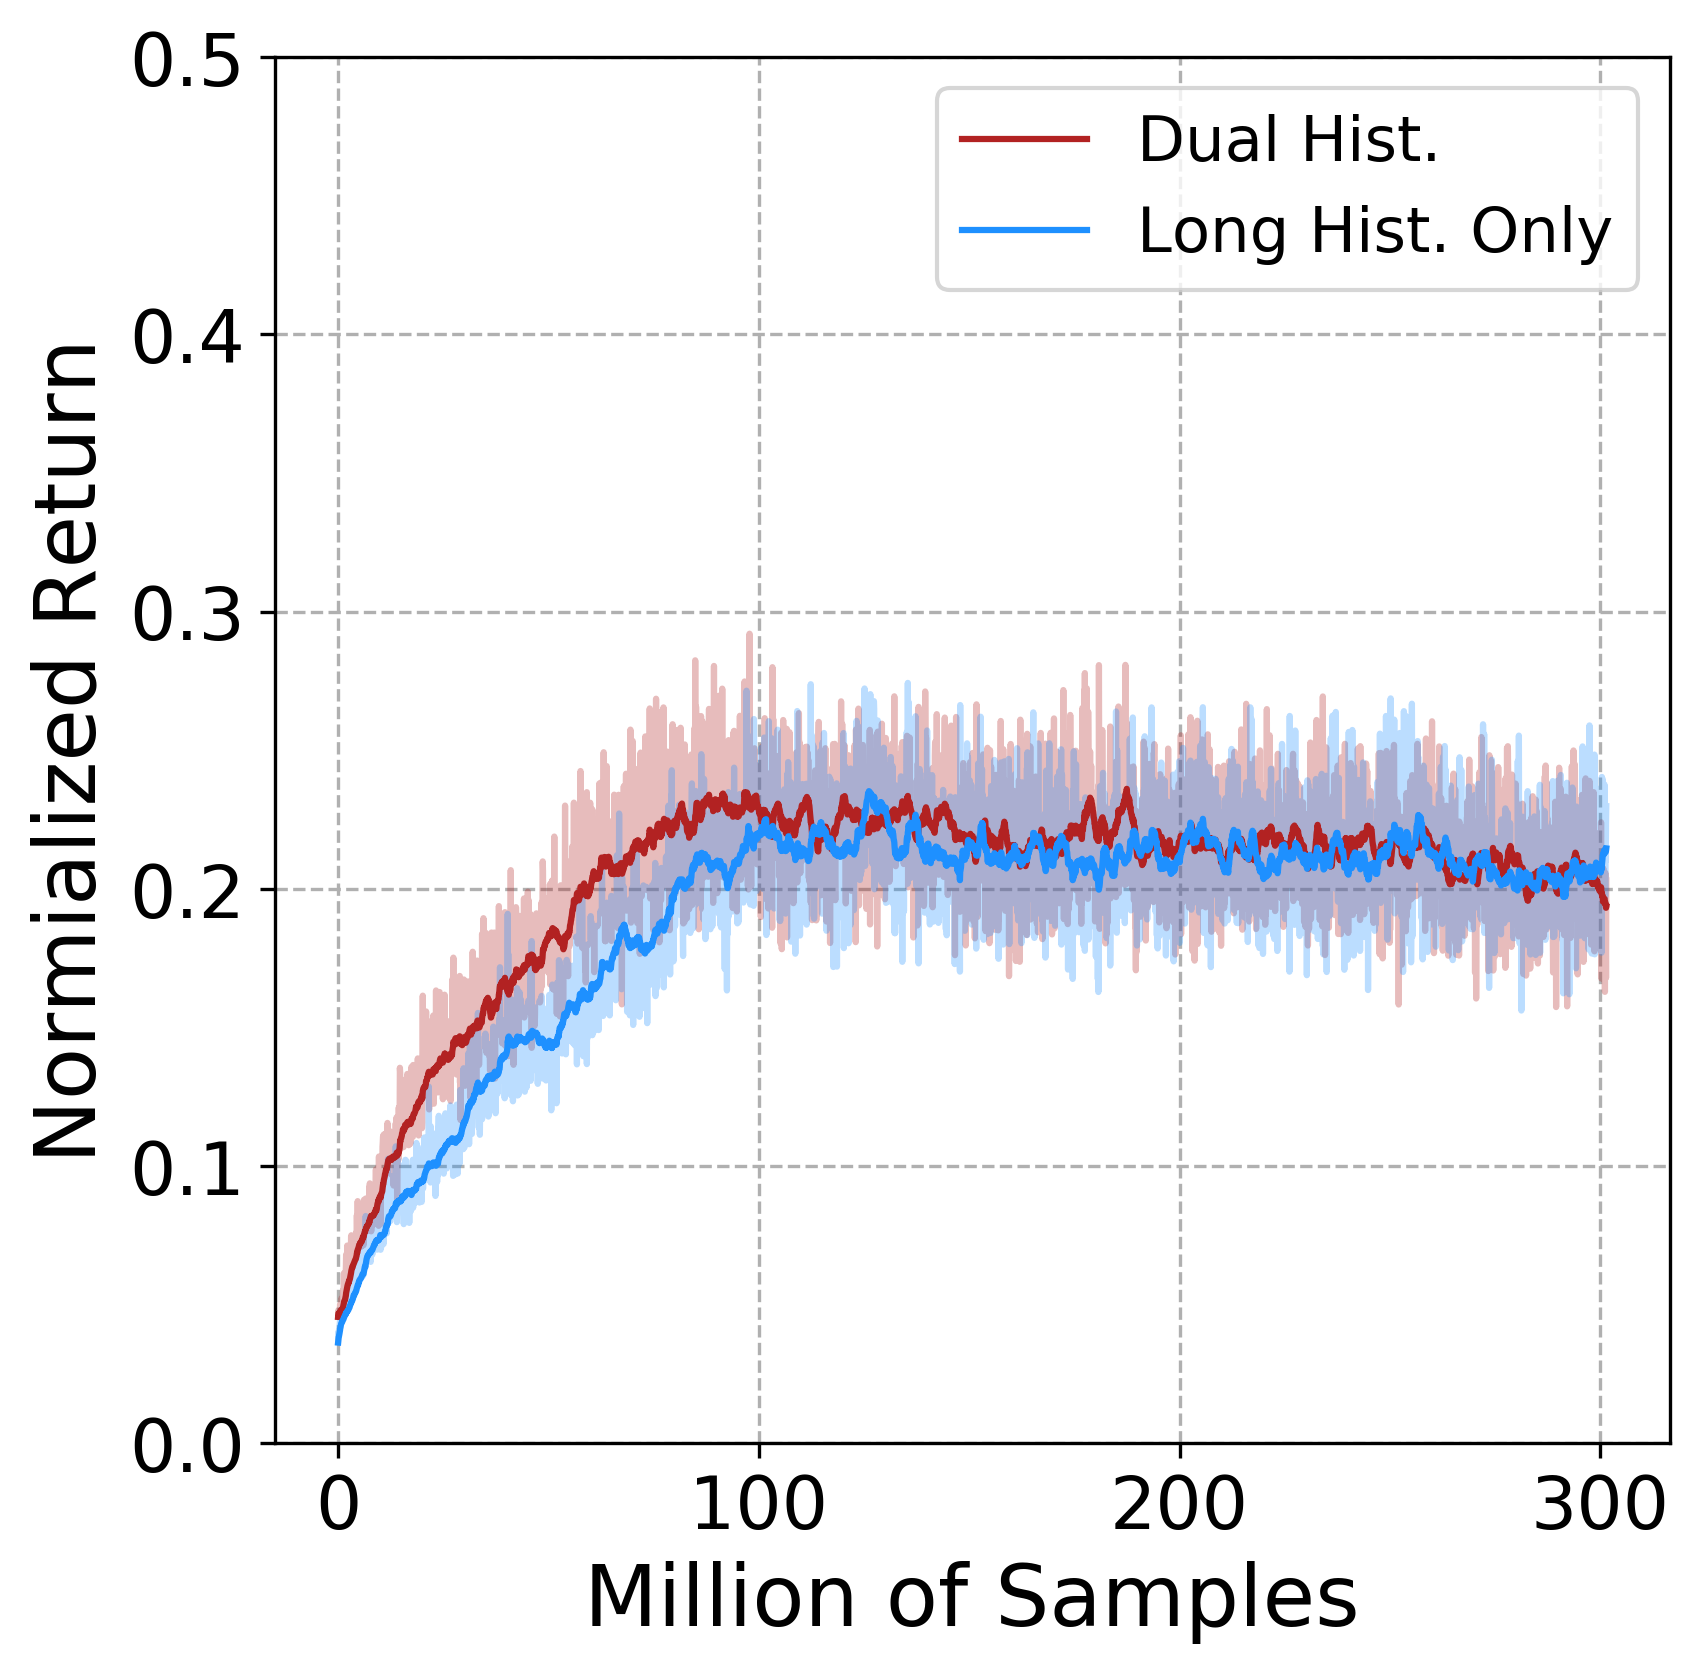
\includegraphics[width=\linewidth]{figures/single_dynrand_lstm_compare_logs_v2.png}
  \caption{LSTM with dual history approach (Dual Hist.) and the LSTM only (Long Hist. Only).}
  \label{subfig:lstm_compare}
\end{subfigure}
\caption{Learning performance using different neural network architectures to encode the robot's I/O history when training a single-task walking policy with dynamics randomization (walking forward at a fixed speed, after finishing single-stage training). For both Long Hist. Only methods, we still provide explicit immediate state feedback alongside the temporal encoder. As shown in Fig.~\ref{subfig:tcn_compare}, using the proposed dual-history approach by providing an explicit short I/O history alongside the TCN encoder, the learning performance is much better than the TCN only. The TCN encodes 2-second robot I/O history and has 3 layers with filter sizes of [34,34,34], a kernel size of 5, a dilation base of 2, and a stride size of 2, with ReLU activation, as suggested in~\cite{lee2020learning}. Fig.~\ref{subfig:lstm_compare} shows that the dual-history approach will not help with the LSTM-based policy. The LSTM encoder has 1 layer of 128 units. However, both TCN with dual-history approach and Long Hist. Only perform better than the LSTM-based policy while using the hyperparameters tuned for LSTM. It suggests that LSTM may only learn to leverage a recent short history and converge to a more suboptimal policy.}
\label{fig:dual_hist_compare}
\end{figure}


\begin{figure}[ht]
\centering
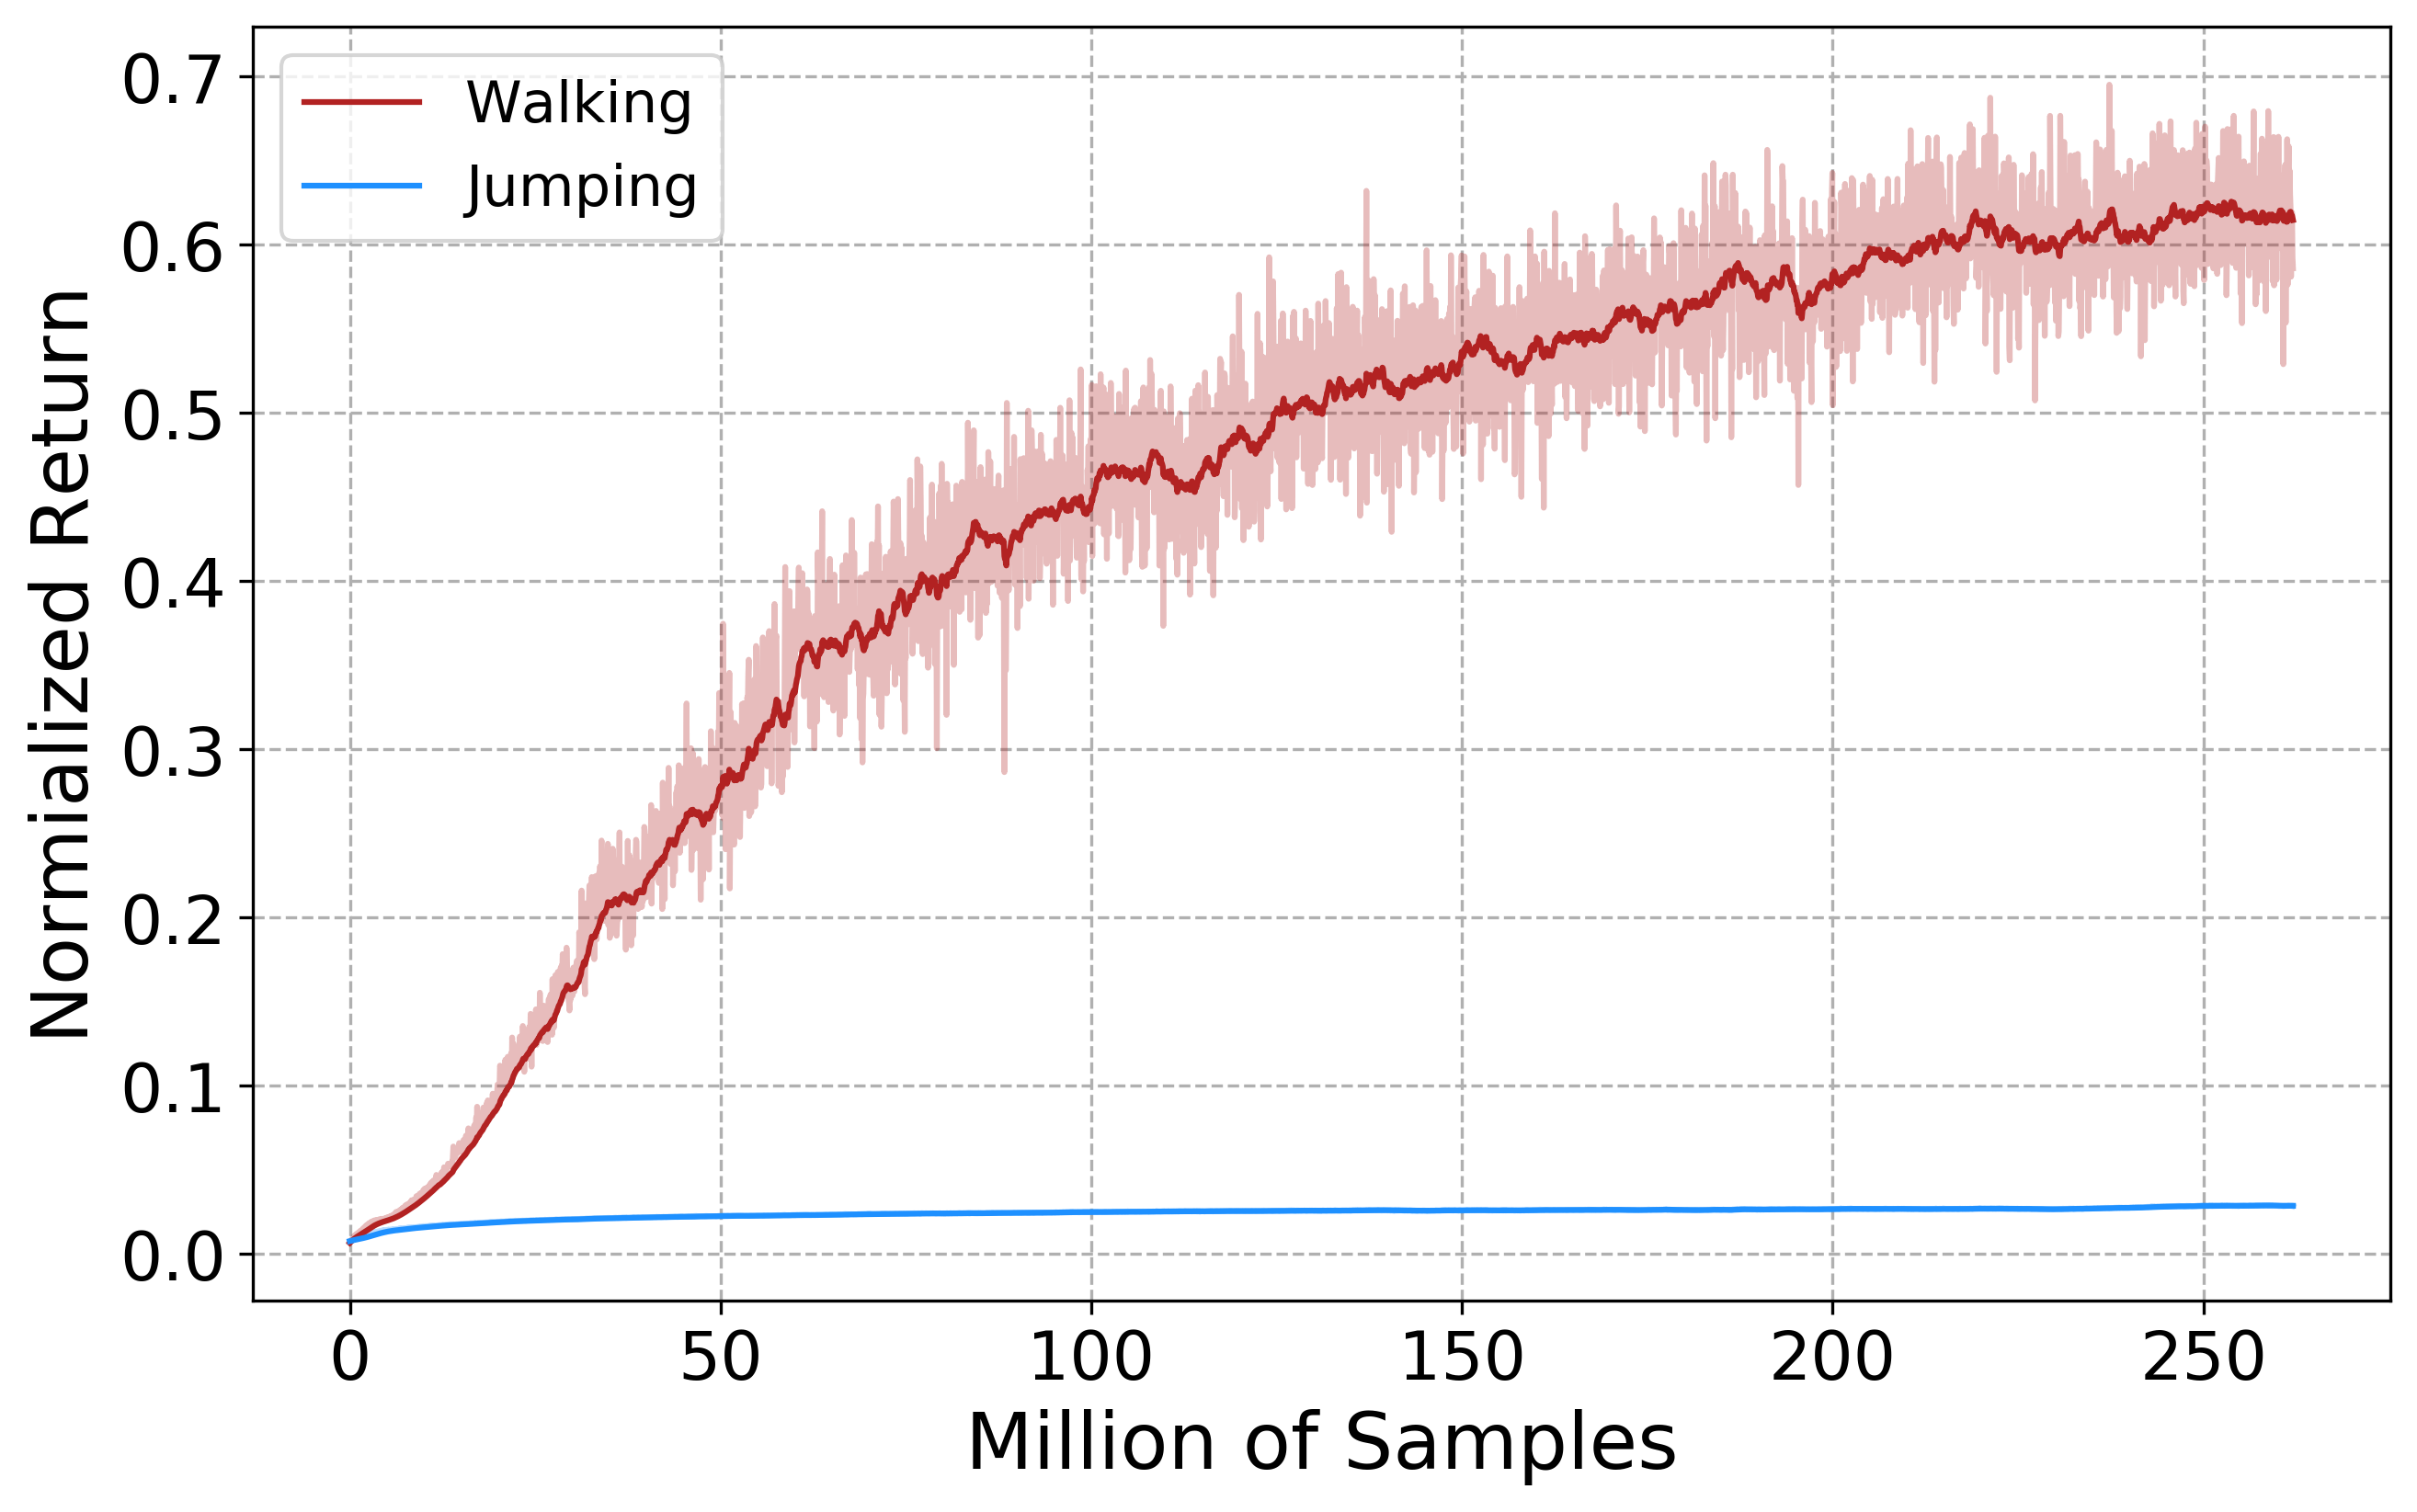
\includegraphics[width=0.75\linewidth]{figures/single_dynrand_lstm_vs_cnn_compare_logs.png}
\caption{Learning performance for training walking (red curve) and jumping (blue curve) skills \emph{from scratch} using the same neural network including the LSTM architecture with the same hyperparamters used in~\cite{siekmann2020learning}. It shows that while the LSTM can learn the walking skill, it may struggle to learn highly dynamic locomotion skills like jumping (shown as a flat curve). This is not to suggest that LSTM cannot learn aperiodic jumping skills, but rather to highlight its sensitivity to hyperparameter tuning across different MDPs (different locomotion skills). This contrasts with the non-recurrent-based policy like the 1D CNN used in this work, which employs a unified set of hyperparameters for all different skills due to the ease of training.}
\label{fig:jump_vs_walk_lstm}
\end{figure}


\begin{figure*}[htp]
\centering
\begin{subfigure}{0.66\linewidth}
  \centering
  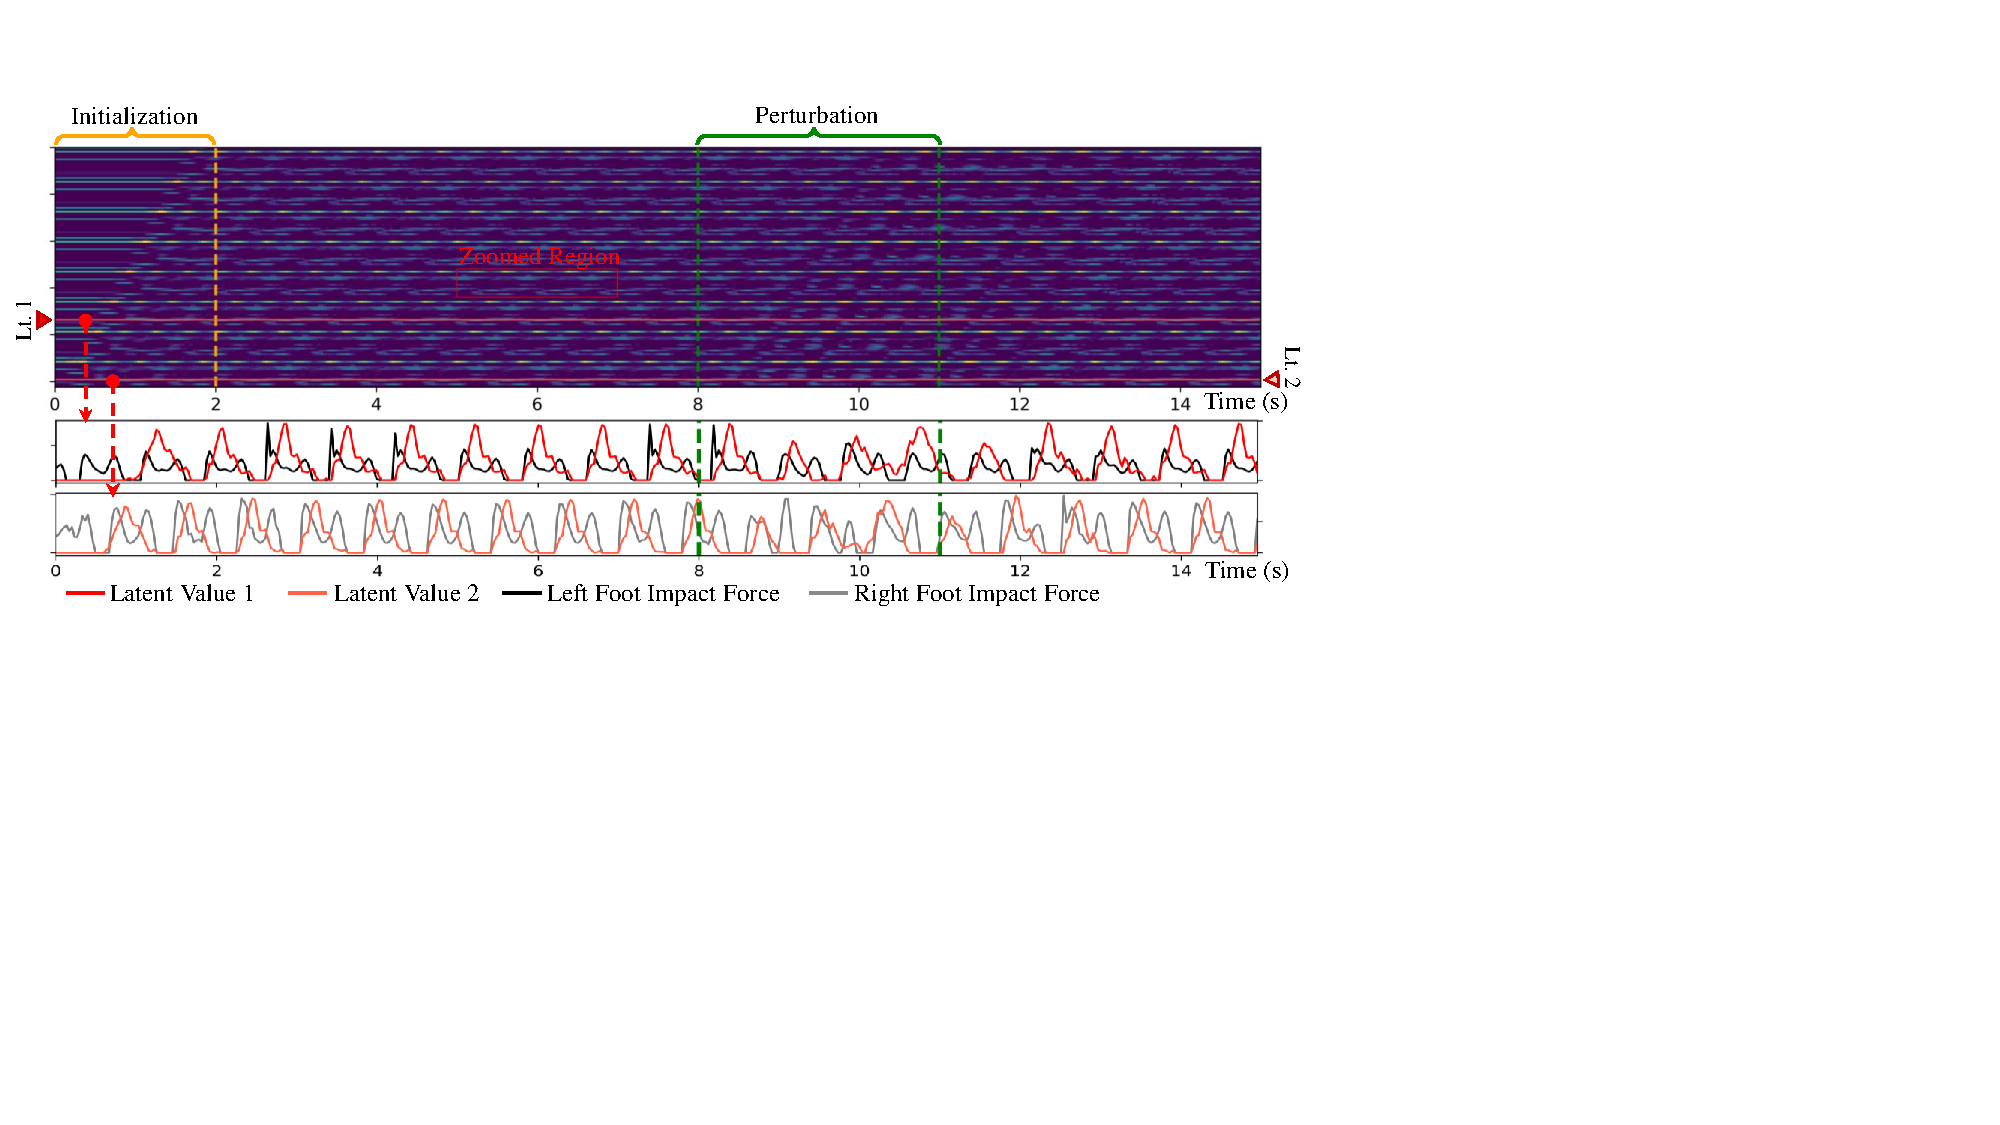
\includegraphics[width=\linewidth]{figures/latent_walk_force.pdf}
  \caption{Recorded latent representation after long-term I/O history encoder during walking. The figure below compares two selected dimensions (marked as red lines) with recorded impact forces on each of the robot's feet.}
  \label{subfig:latent_walk_force}
\end{subfigure}
\begin{subfigure}{0.33\linewidth}
  \centering
  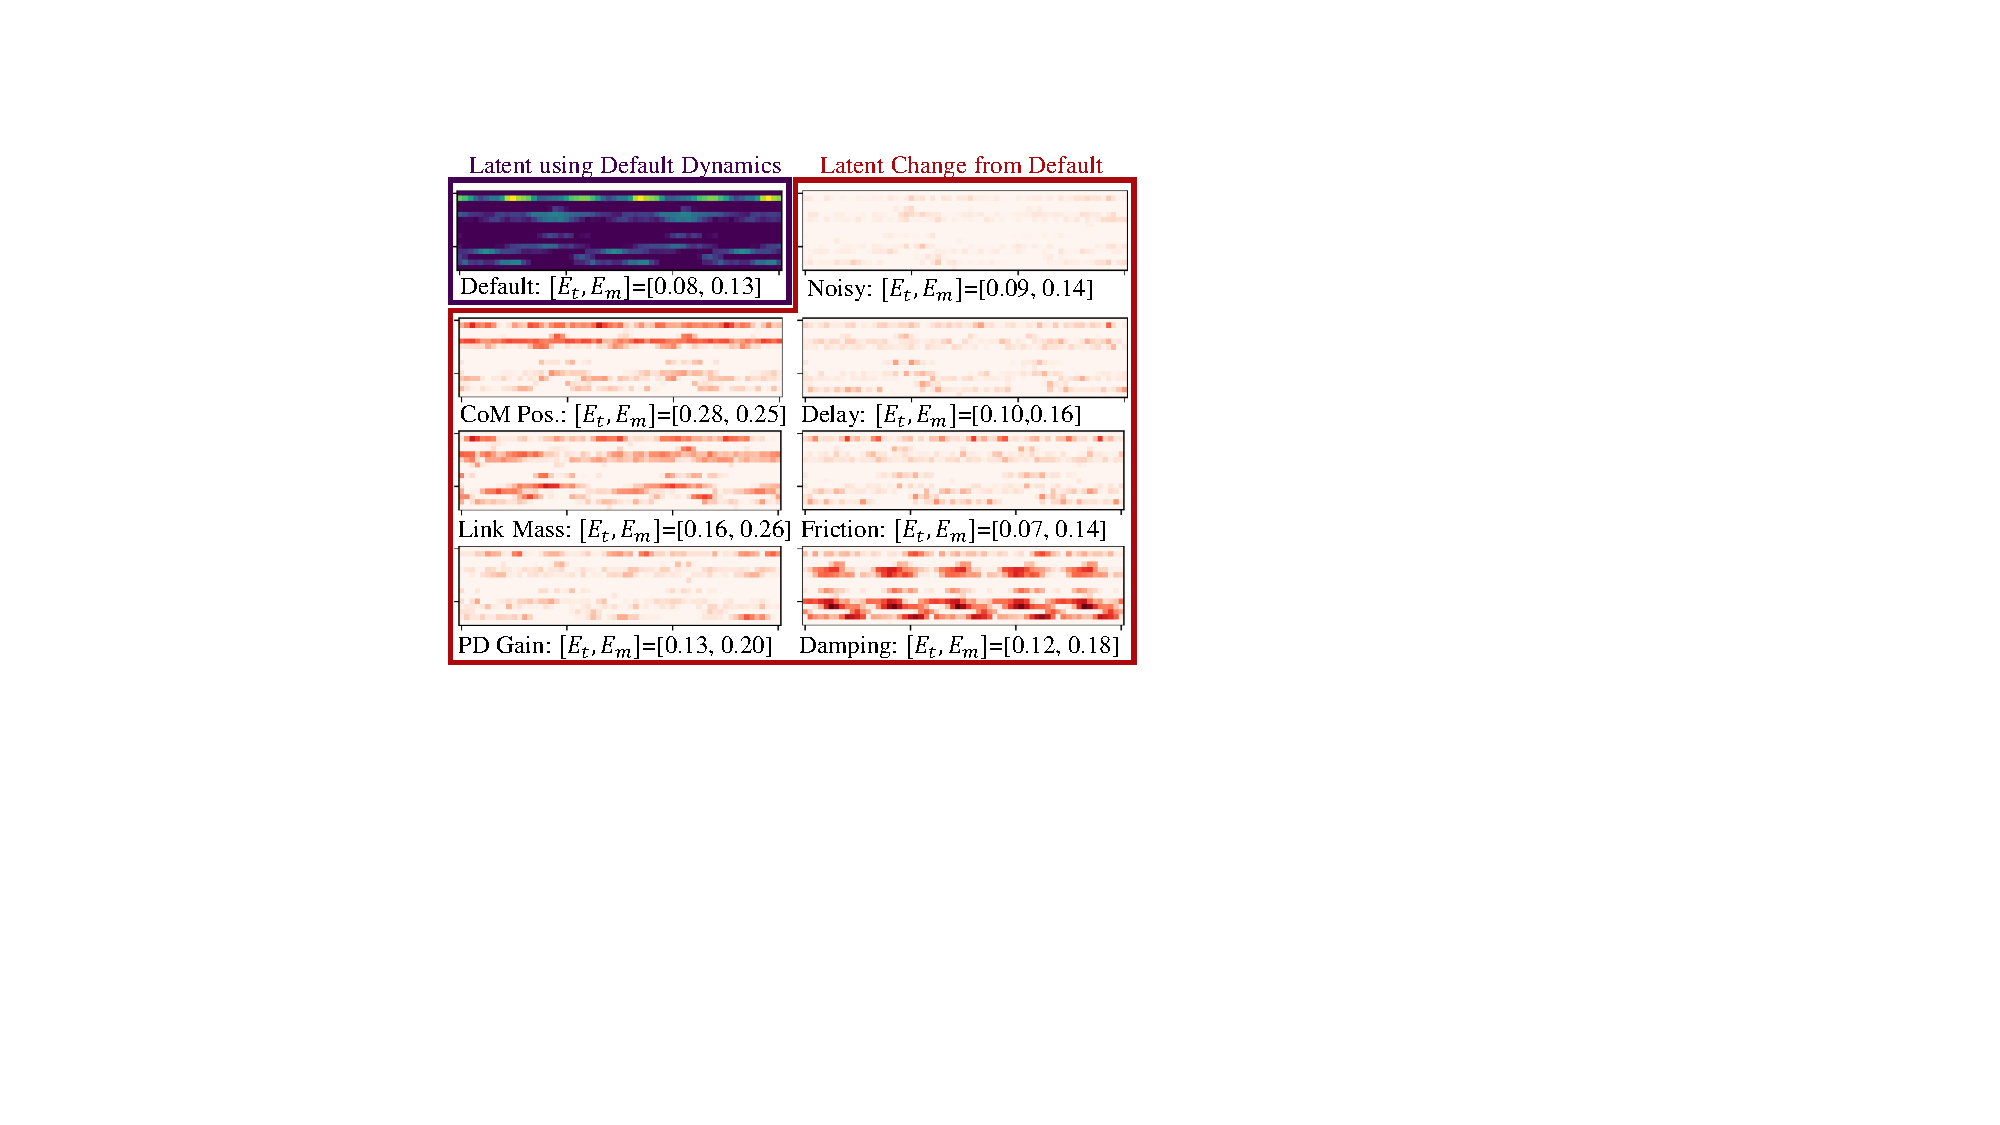
\includegraphics[width=\linewidth]{figures/latent_walk_zoomed_delta.pdf}
  \caption{The blue plot shows the robot's latent representation with default dynamics parameters during walking. The red plots indicate changes in the same region under different dynamics.}
  \label{subfig:latent_walk_zoomed}
\end{subfigure}
\caption{Adaptivity test on the obtained walking policy in simulation (MuJoCo). The robot is commanded to walk forward at 0.6 m/s with no lateral or turning movement at normal height (0.95 m). Fig.~\ref{subfig:latent_walk_force} records the latent embedding after the policy's long I/O history encoder over 15 seconds. An external backward perturbation force of 30 N is applied on the robot base from 8 to 11 seconds. We can observe the changes in the latent embedding with the existence of the perturbations. The image below shows a strong correlationship between the two selected latent dimensions with the robot's impact force or contact event. Fig.~\ref{subfig:latent_walk_zoomed} shows the change of the latent embedding (the same zoomed region marked as the red bounding box in Fig.~\ref{subfig:latent_walk_force}) with respect to the change of different dynamics parameters during the same walking task. These ablation studies are the same as running conducted in Fig.~\ref{subfig:latent_run_zoomed}. The control performance metrics, tracking error $E_t$ and motion tracking error $E_m$, show small changes with a large change in the dynamics parameters.}\label{fig:latent_vis_walking}
\end{figure*}



\begin{figure*}[htp]
\centering
\begin{subfigure}{0.49\linewidth}
  \centering
  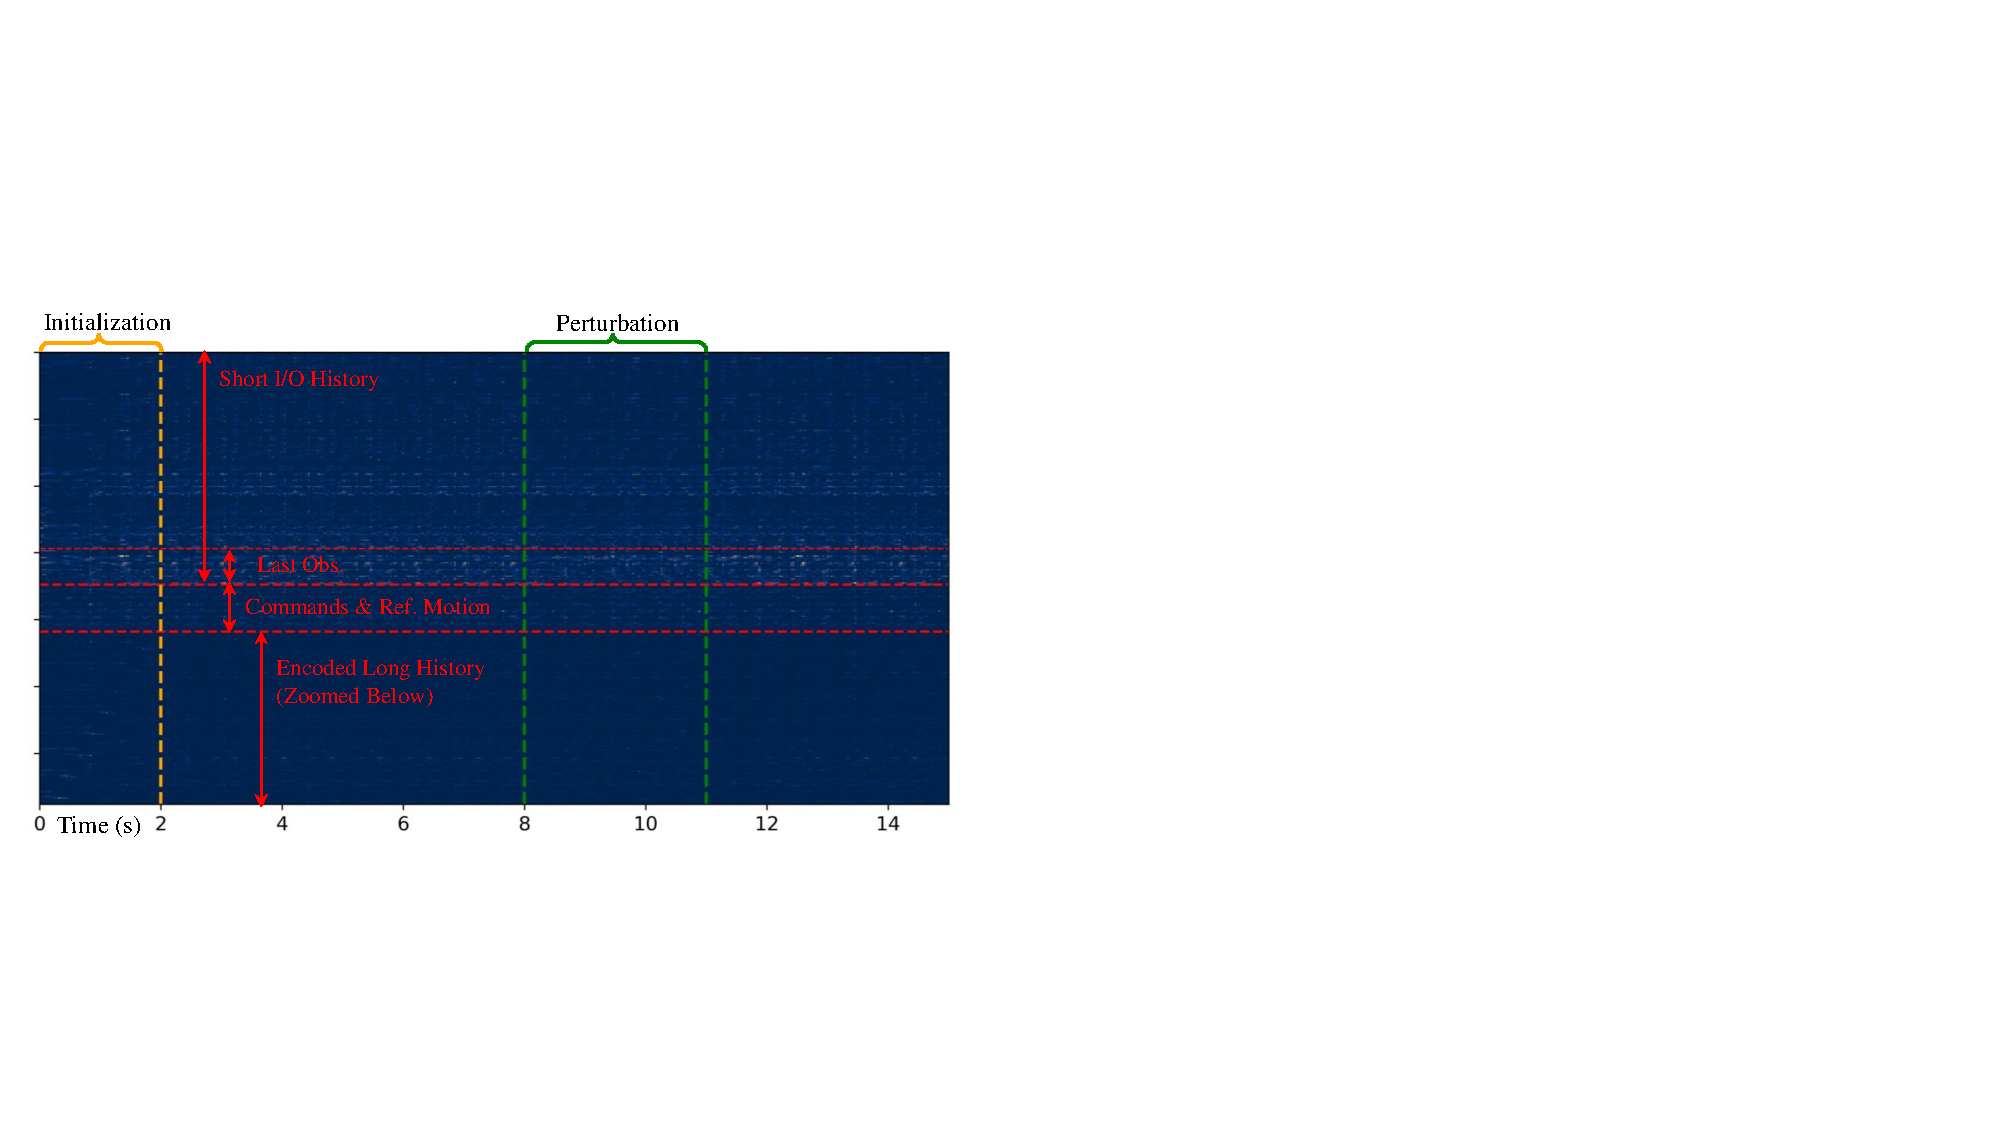
\includegraphics[width=\linewidth]{figures/run_saliency_all.pdf}
  \caption{Running}
  \label{subfig:run_saliency_all}
\end{subfigure}
\begin{subfigure}{0.49\linewidth}
  \centering
  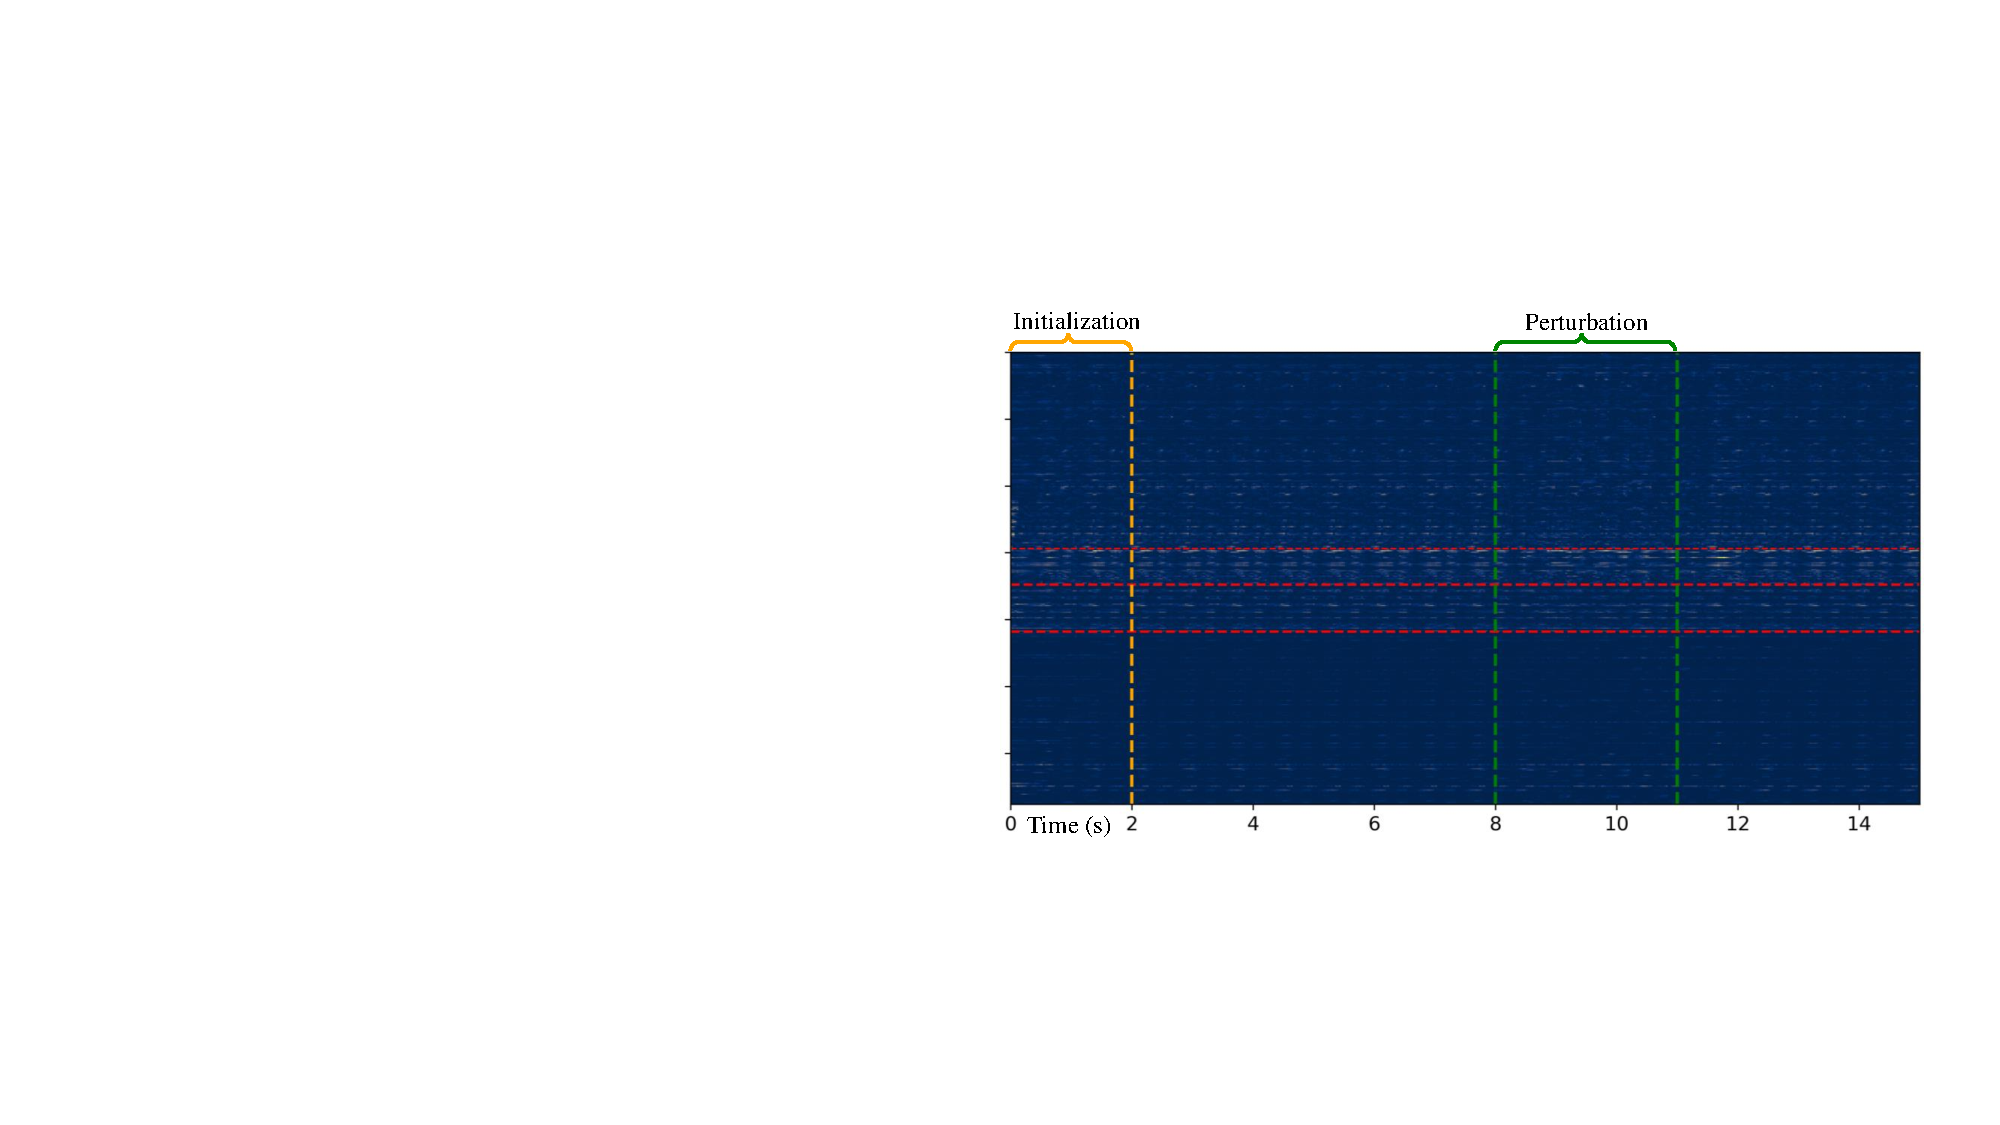
\includegraphics[width=\linewidth]{figures/walk_saliency_all.pdf}
  \caption{Walking}
  \label{subfig:walk_saliency_all}
\end{subfigure}
\begin{subfigure}{0.485\linewidth}
  \centering
  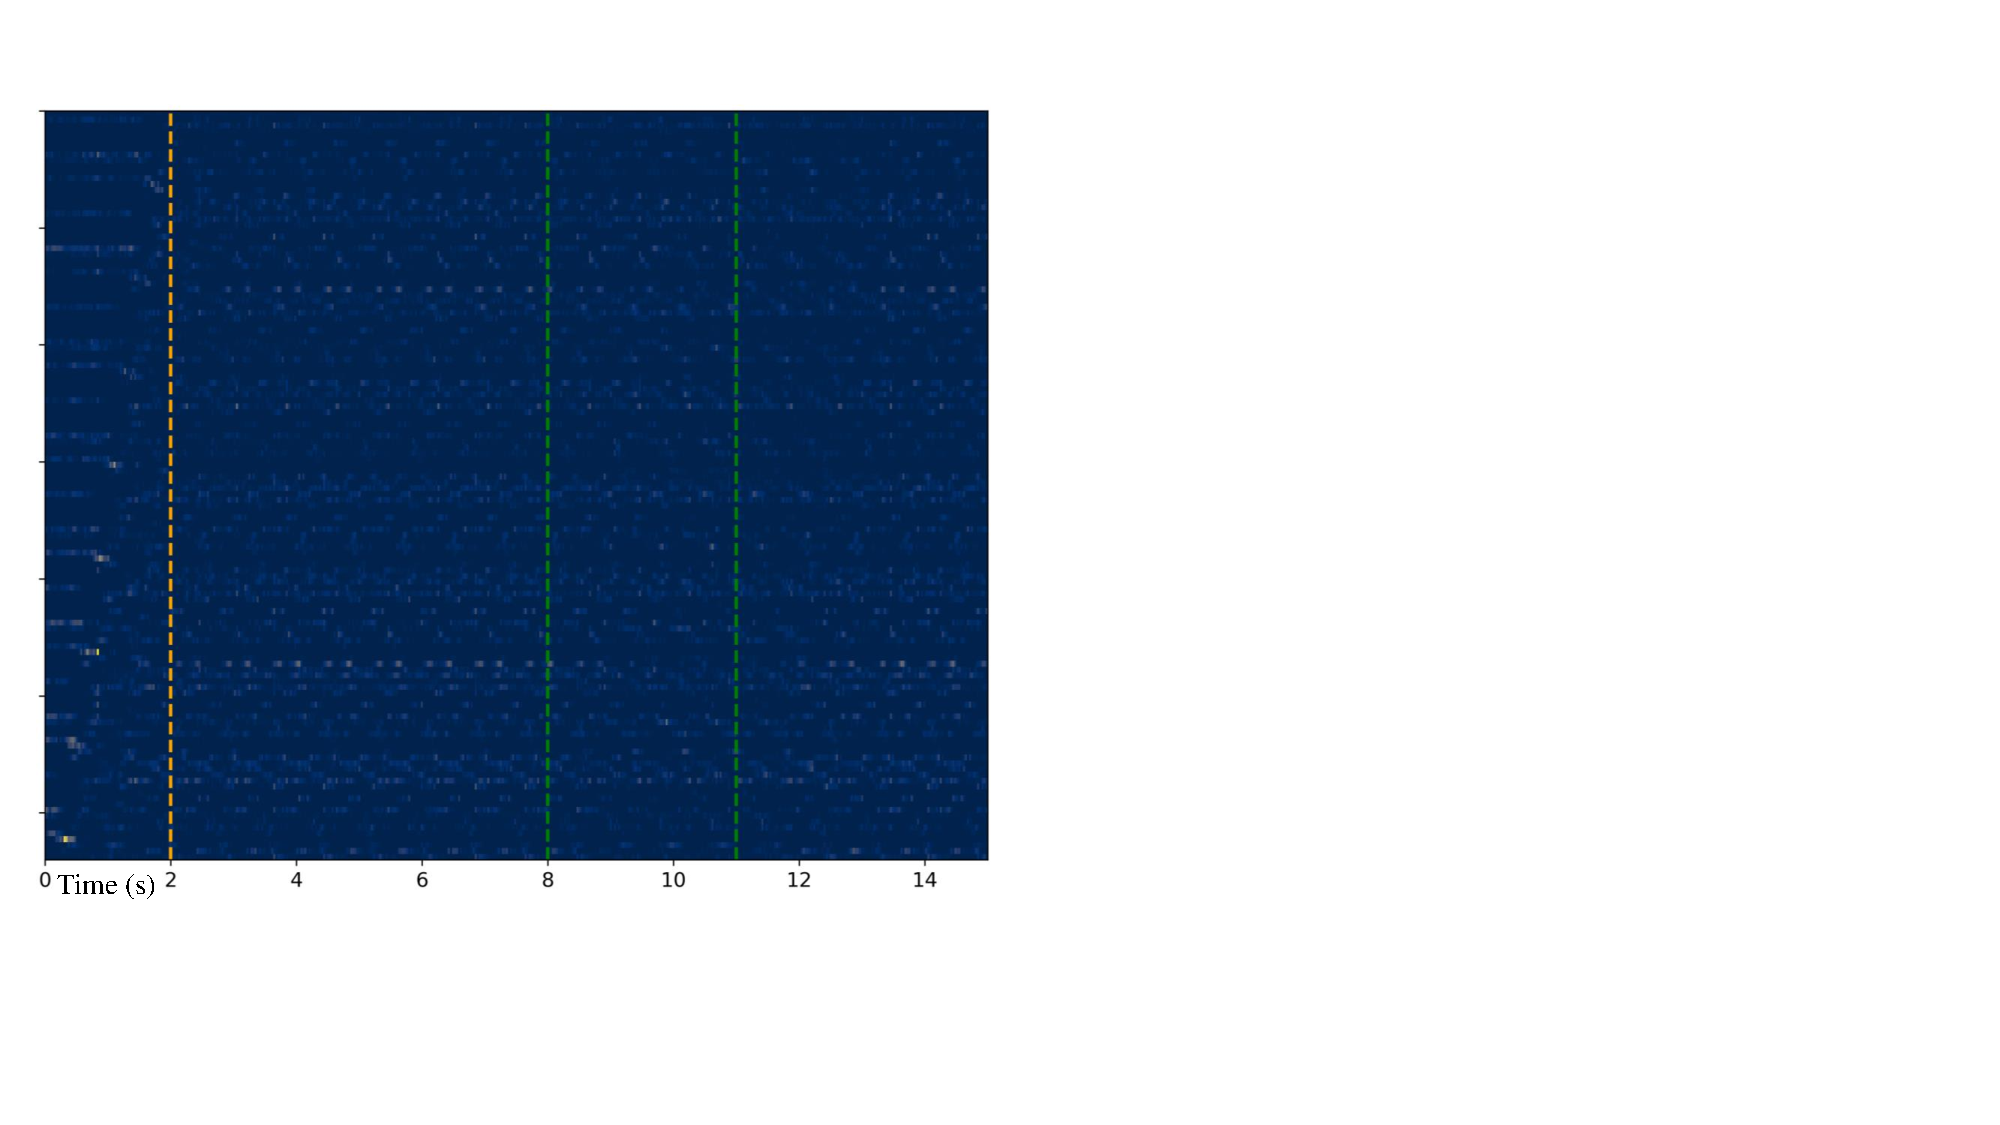
\includegraphics[width=\linewidth]{figures/run_saliency.pdf}
  \caption{Zoomed Region (Encoded Long History) of Running}
  \label{subfig:run_saliency}
\end{subfigure}
\begin{subfigure}{0.49\linewidth}
  \centering
  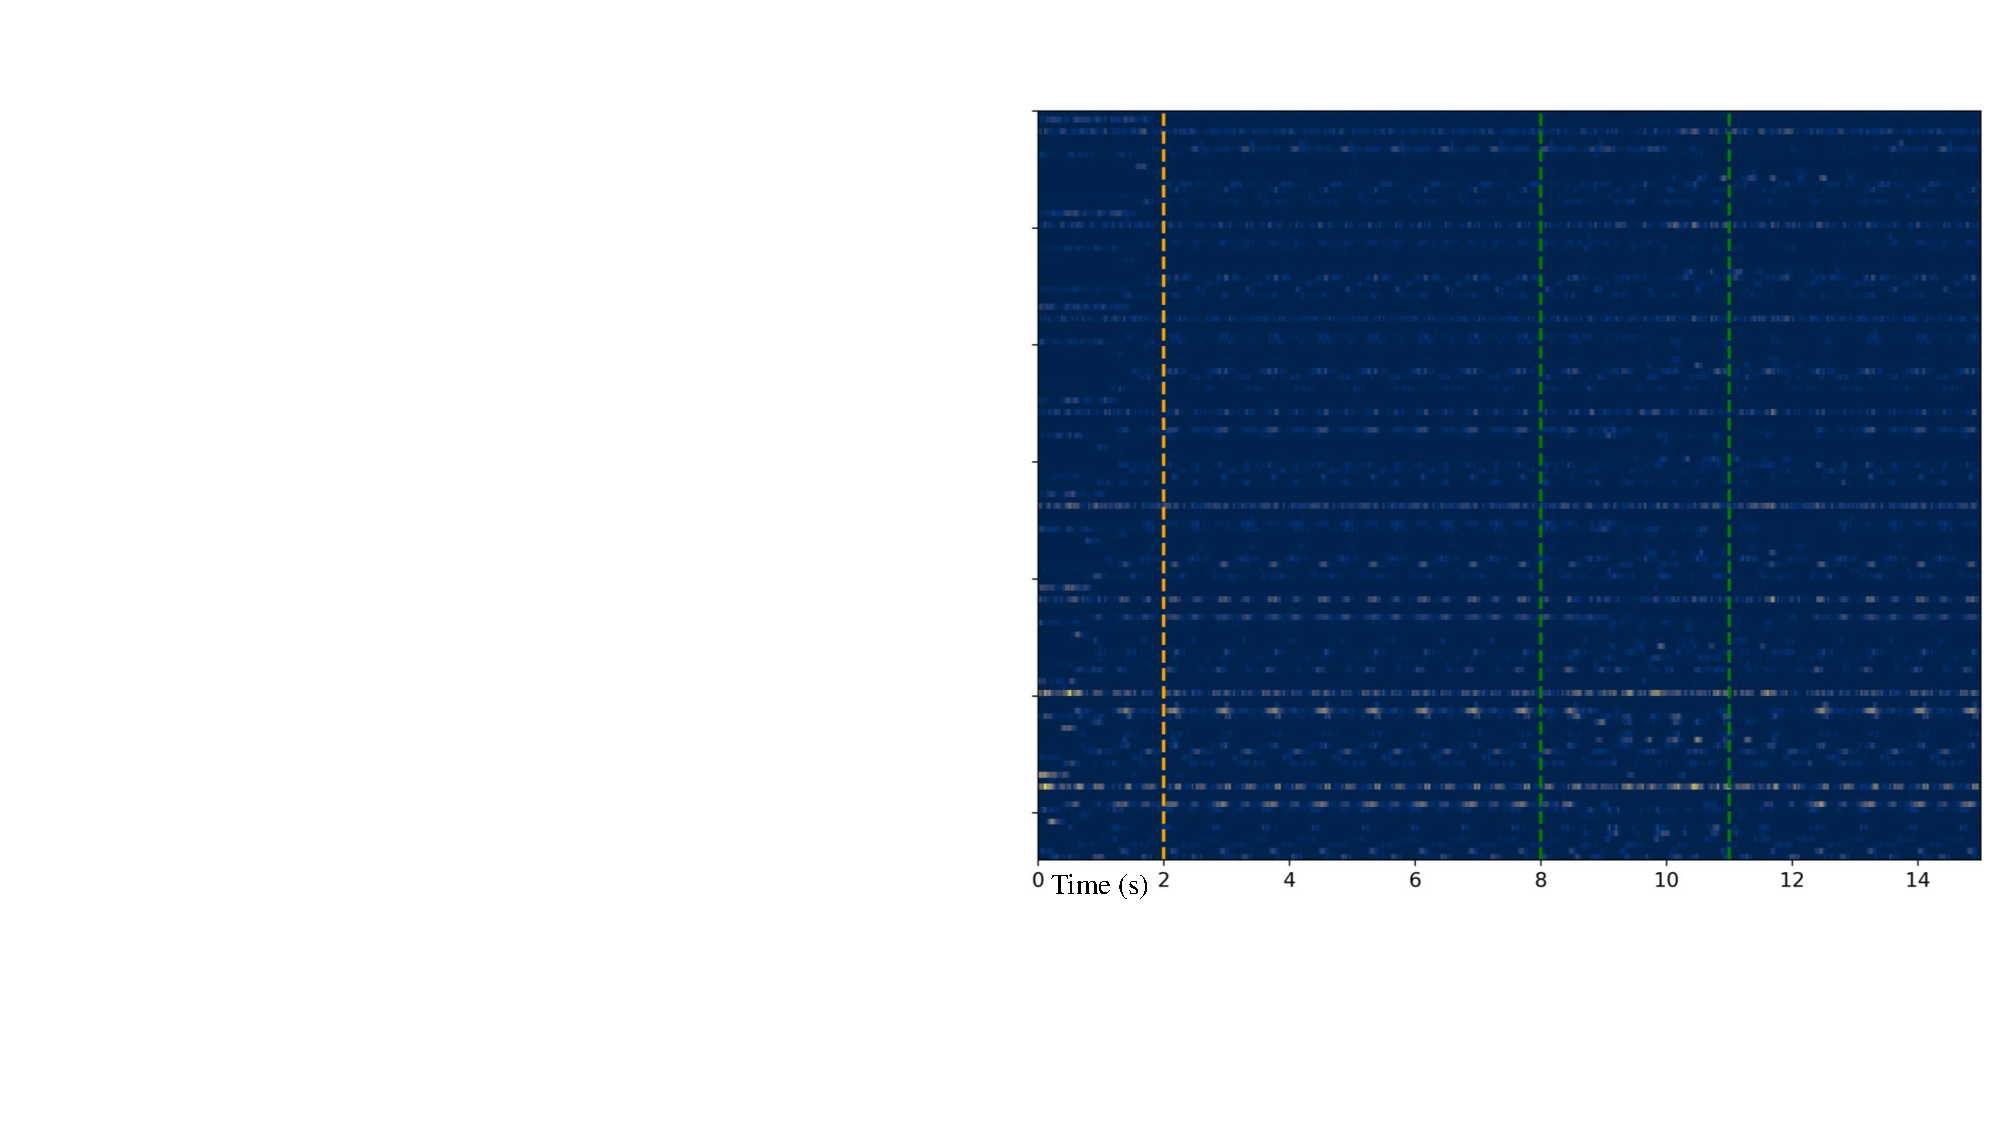
\includegraphics[width=\linewidth]{figures/walk_saliency.pdf}
  \caption{Zoomed Region (Encoded Long History) of Walking}
  \label{subfig:walk_saliency}
\end{subfigure}
\caption{The saliency map of the MLP base with respect to the entire input while the robot is (a) running or (b) walking with the existence of a perturbation from 8 to 11 seconds in a 15-second test. The zoomed regions of the saliency map w.r.t. latent embedding from the long history encoder are shown in detail in (c) for running and (d) for walking. These are the same tests reported in Fig.~\ref{fig:latent_vis} and Fig.~\ref{fig:latent_vis_walking}. The pixels with a lighter color represent the MLP base focus more on this value (higher saliency). These maps show that the MLP base, which produces the policy action, focuses more on the short I/O history, especially the latest observation, highlighting the importance of short I/O history in the input. Moreover, if we take a close look at the encoded long I/O history (c,d), the robot can also focus on different regions of the latent embedding to deal with the change in environments and therefore adjust its output. Therefore, it indicates that the inclusion of long I/O history is also beneficial, which also provides insights on the benchmark conducted in Fig.~\ref{fig:dynrand_three}.}\label{fig:saliency_map}
\end{figure*}

We conducted an ablation study to investigate the effects of varying history lengths on a non-recurrent policy that explicitly requires a specified history length. Using bipedal running training as an example, Fig.~\ref{fig:hist_compare} illustrates the learning performance of training a single-task running policy (which has completed the first-stage training) with extensive dynamics parameters and varying lengths of robot I/O history.

As suggested by Fig.~\ref{fig:hist_compare}, increasing the history length, such as from 1 second to 2 seconds, or from 2 seconds to 3 seconds, consistently enhances learning performance. This improvement occurs because a longer I/O history provides more information on the robot's dynamics parameters, aiding in better state estimation. However, continually extending the history length may not always be beneficial, as it can introduce redundant information that the robot must filter out. This is evidenced by a drop in learning performance when history length increases from 3 seconds to 4 seconds, as shown in Fig.~\ref{fig:hist_compare}. 
In bipedal locomotion control, where remembering events that happened further earlier is less crucial, a longer history could lead more training samples for the robot to distill useful information. 
Therefore, we recommend using a history length that spans a relatively short timespan, such as the 2 seconds used in this work, for more stable training and relatively good performance in learning bipedal locomotion control. For readers interested in adopting this method for their robots, finding the optimal history length could be beneficial for specific tasks, but we suggest starting with a 2-second history, which has been tested extensively in this work.


}



\subsection{Comparison of Use of Different Temporal Encoders}\label{appendix:lstm_tcn}






To explore the effects of different neural network structures encoding the robot's I/O long history, we conducted an ablation study and benchmarked policies based on TCN and LSTM. TCN, a non-recurrent structure that encodes temporal information, is used in~\cite{lee2020learning}, while LSTM, a recurrent structure, is utilized in other bipedal locomotion control works like~\cite{siekmann2020learning}. To eliminate potential confounding factors such as poor implementation, we adopted the training algorithms (PPO and recurrent PPO) and training hyperparameters open-sourced from~\cite{siekmann2020learning}, which underpin many subsequent studies such as~\cite{siekmann2021blind, siekmann2021sim, crowley2023optimizing}. The MDP design (training environment) employed the walking and jumping scenarios developed in this work.

As shown in Fig.~\ref{subfig:tcn_compare}, providing the base policy with a short 4-timestep I/O history alongside the TCN encoder significantly improves learning performance compared to using TCN alone (while still providing the base policy with immediate last state feedback, which is the form used in \cite{lee2020learning}). This suggests that the dual-history approach can consistently enhance learning performance for non-recurrent structures that encode an explicit history length. Note that in this comparison, we use the same TCN implementation as detailed in Table S5 in~\cite{lee2020learning}.

Conversely, as depicted in Fig.~\ref{subfig:lstm_compare}, the LSTM-based policy shows no significant improvement whether a short history is provided or not. Additionally, it tends to converge to a lower return plateau compared to the TCN-based policy, even though the TCN used hyperparameters tuned for LSTM. This might indicate that LSTM encoders may learn to focus more on recent short history and pay less attention to older history. Although LSTM hidden states are only reset at episode ends, they may quickly converge to a suboptimal policy focusing primarily on recent history, explaining why providing additional short history does not enhance performance and why LSTM underperforms compared to TCN that was explicitly trained to utilize a long history. This observation aligns with findings reported in~\cite{lee2020learning} and \cite{singh2023learning}.

Moreover, extending the LSTM-based policy to learn jumping skills resulted in training failure, even using the same architecture and hyperparameters from~\cite{siekmann2020learning} that reproduced the same walking skill developed in this work, as illustrated in Fig.~\ref{fig:jump_vs_walk_lstm}. Please note that we are not asserting that it is impossible for LSTM to learn aperiodic skills like jumping, but it is difficult without carefully tuning hyperparameters during training. 
In contrast, our method provides a straightforward and general approach for learning various skills, using unified hyperparameters across all tasks. After finalizing the training for walking, we did not adjust any hyperparameters for jumping or running.

In summary, the dual history approach consistently helps learning performance for policies recording explicit robot history (non-recurrent policies like TCN and 1D CNN), but does not improve recurrent policies like LSTM. Moreover, recurrent policies are sensitive to hyperparameter tuning across different MDPs (such as locomotion control) and may more readily converge to suboptimal policies. Therefore, dual-history-based non-recurrent policy could be more favorable for bipedal locomotion control cases. 







\subsection{Latent Visualization of Walking Policy}\label{appendix:walking_latent}
The results of adaptivity test on the obtained walking policy by the proposed method are presented in Fig.~\ref{fig:latent_vis_walking}. 
The adaptivity test is similar to the ones conducted on the running policy discussed in Sec.~\ref{subsec:adaptivity}. 
It evaluates the change of latent embedding after the long I/O history encoder when the robot is commanded to walk at a constant forward speed of 0.6 m/s. 
The findings are consistent with the ones observed from the tests on other skills reported in Sec.~\ref{subsec:adaptivity}: we show that the latent embedding is able to capture the time-variant changes like external perturbation and contact events (Fig.~\ref{subfig:latent_walk_force}) and time-invariant dynamics shifts (Fig.~\ref{subfig:latent_walk_zoomed}). 
During the ablation study on the dynamics shifts, the latent embedding differs when dynamics parameters change, but the resulting control performance shows little change. This indicates the adaptivity of the walking policy.  





\subsection{Saliency Map}\label{appendix:saliency}
To further understand how the policy adjusts its action based on the environment changes, we visualize the saliency map in Fig.~\ref{fig:saliency_map} as used in~\cite{lee2020learning}. The saliency map reflects how important each input dimension is to the neural network output (\textit{i.e.}, where does the policy focus).


As shown in the saliency map of the MLP base, which produces the final policy action on the entire input, the robot focuses more on the short I/O history, particularly the most recent observation, highlighting the importance of the short I/O history, during both running (Fig.~\ref{subfig:run_saliency_all}) and walking (Fig.~\ref{subfig:walk_saliency_all}).

We can take a close look at the zoomed regions (encoded long history) of the entire saliency map in the same test of the running (Fig.~\ref{subfig:latent_run_force}) and walking (Fig.~\ref{subfig:latent_walk_force}). The saliency maps with respect to the encoded long history have different focuses on different parts of the embeddings from the long-history encoder with the existence of the external perturbation during running (Fig.~\ref{subfig:run_saliency}) or walking (Fig.~\ref{subfig:walk_saliency}). 
This further suggests that the proposed RL policy could utilize the long history information to adjust the action for different control scenarios, \textit{i.e.}, the long I/O history is useful. 


From the extensive ablation study in Fig.~\ref{fig:dynrand_three}, we observed differences in learning performance and sim-to-real transfer depending on the use of history.
It will result in degradation by either removing the short I/O history, even keeping the most recent observation that drew the most attention, which is Long History Only in Fig.~\ref{fig:benchmark}d, or removing the long I/O history (Short History Only, Fig.~\ref{fig:benchmark}e). These saliency maps on the entire input space provide insights into the reason behind this.




\subsection{Errors of Estimator in High-Speed Running}\label{appendix:estimaion_error}

In this section, we present the estimation errors of the state estimator (EKF) we used in the high-speed running. In Fig.~\ref{fig:state_est_err}, we compare the robot ground-truth sagittal velocity $\dot{q}_x$ during running obtained from simulation and the corresponding estimated velocity from the estimator. During high-speed running (larger than 3 m/s), we observe a large estimation error from the estimator to which we only have access during real-world experiments. This suggests that the robot's actual running speed in the real world is faster than the recorded estimated speed, and may be the upper envelope of the estimation. This large estimation error is further supported when comparing the estimated speed and the robot's actual average speed (traveled distance/elapsed time). These suggest a smaller actual tracking error during high-speed running than the experiment logs suggested. This also suggests the necessity of including this estimator during training rollout to let the robot train with the observation data produced by this inaccurate estimator. But still, the robot tends to have a noticeable tracking error during running in the high-speed region due to the sim-to-real gap and robot hardware limitation. We note that developing a reliable state estimator for dynamic bipedal locomotion skills using RL could be an interesting future work.



\begin{figure}[!]
\centering
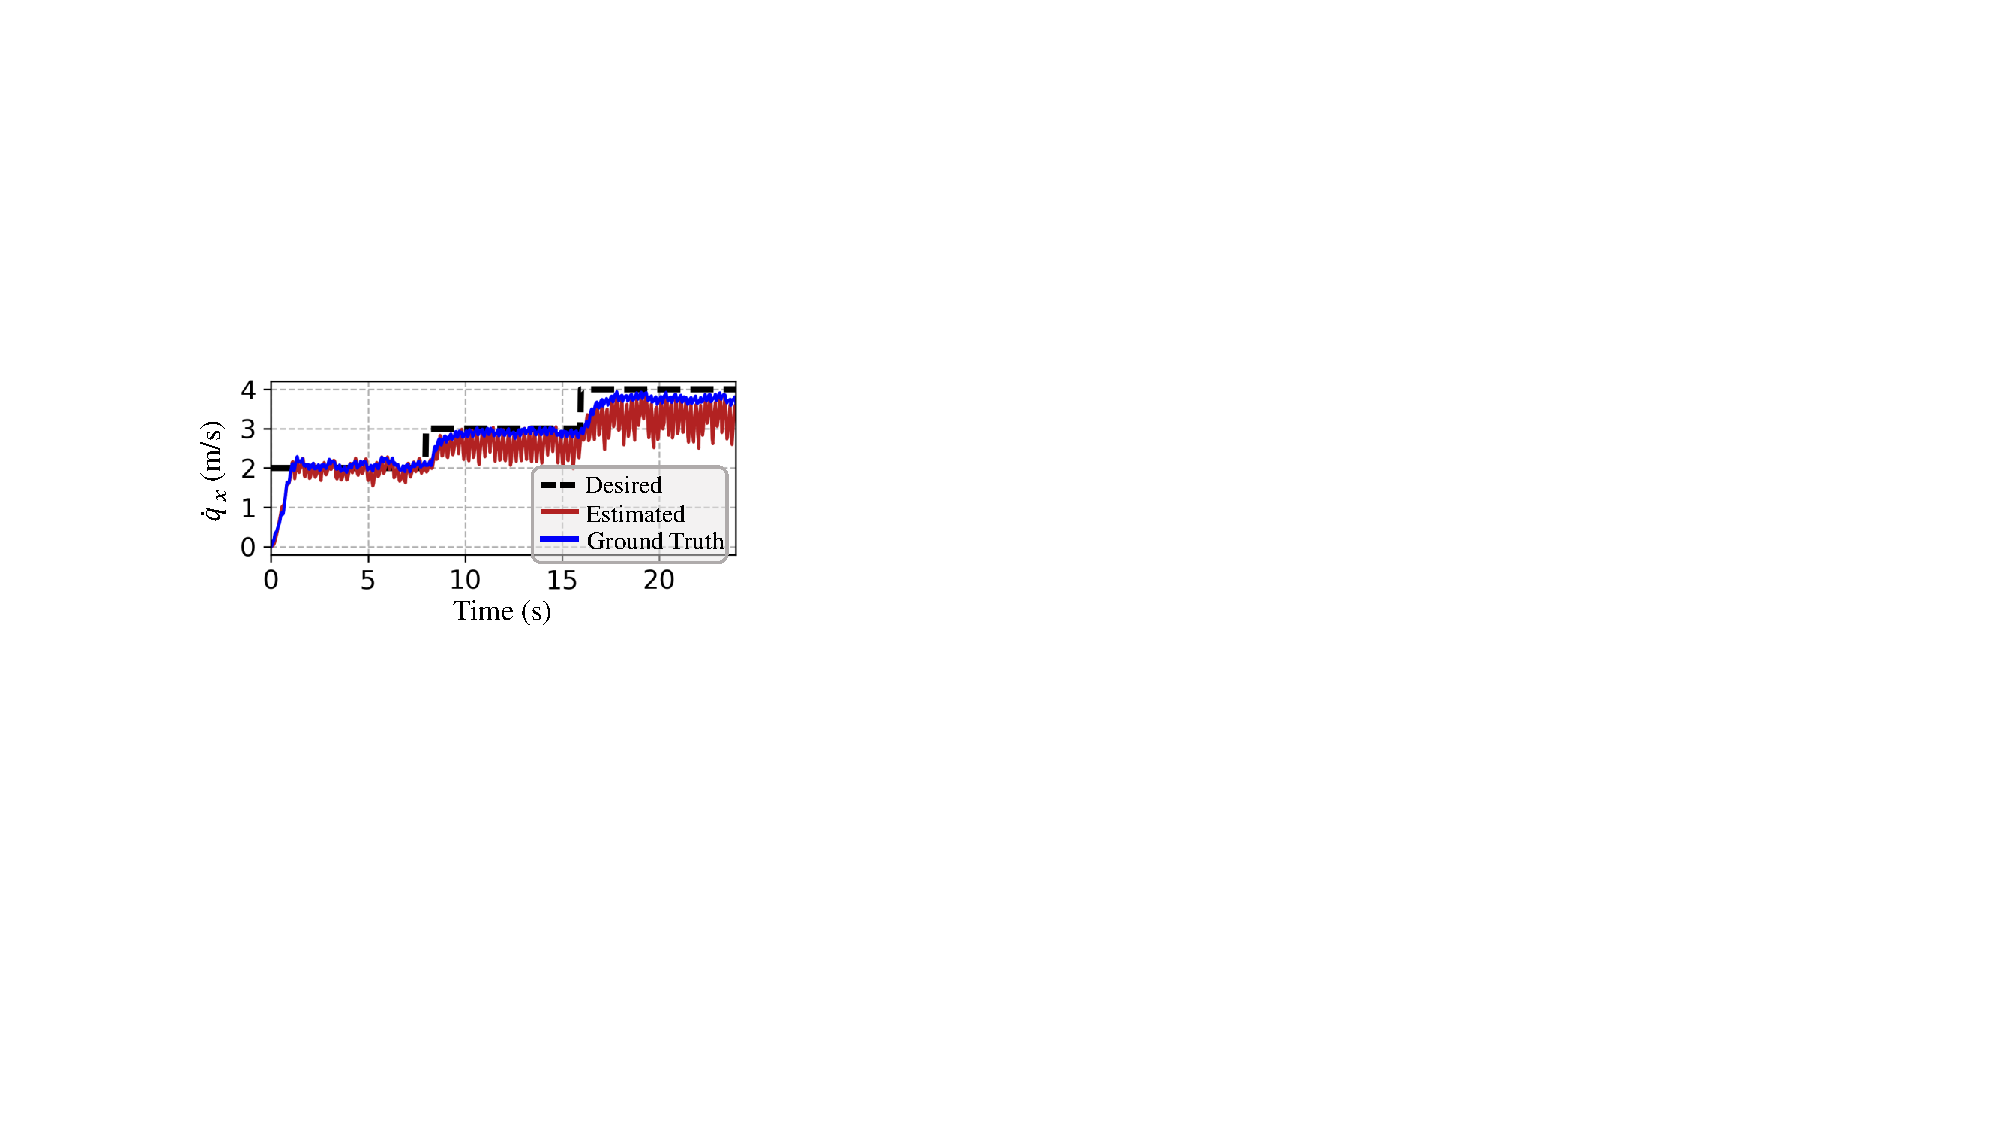
\includegraphics[width=0.8\linewidth]{figures/state_est_compare.pdf}
\caption{The large estimation error using the robot onboard velocity estimator (based on EKF) during high-speed running \emph{in simulation}. In this figure, the robot is controlled by the proposed running policy to track variable commands (black dashed line) in simulation, the estimated sagittal velocity $\dot{q}_x$ is recorded as the red line while the robot's actual running speed is recorded as the blue line. \emph{The ground-truth speed is obtained from the simulator}. Although showing accurate results under slow speed (such as 2 m/s), the estimated velocity shows a significant error in the high-speed region (above 3 m/s) compared to the ground-truth speed. The robot's actual speed tends to be the upper envelope of the estimated speed. In real-world experiments, we only have access to the state estimator whose result we can report, such as the running speed tracking results in Fig.~\ref{subfig:run_400_log}. This comparison shows that the robot's actual running speed in the real world is faster than the reported estimated value and closer to the command.}\label{fig:state_est_err}
\end{figure}



\begin{figure}[!htp]
\centering
\begin{subfigure}{0.455\linewidth}
  \centering
  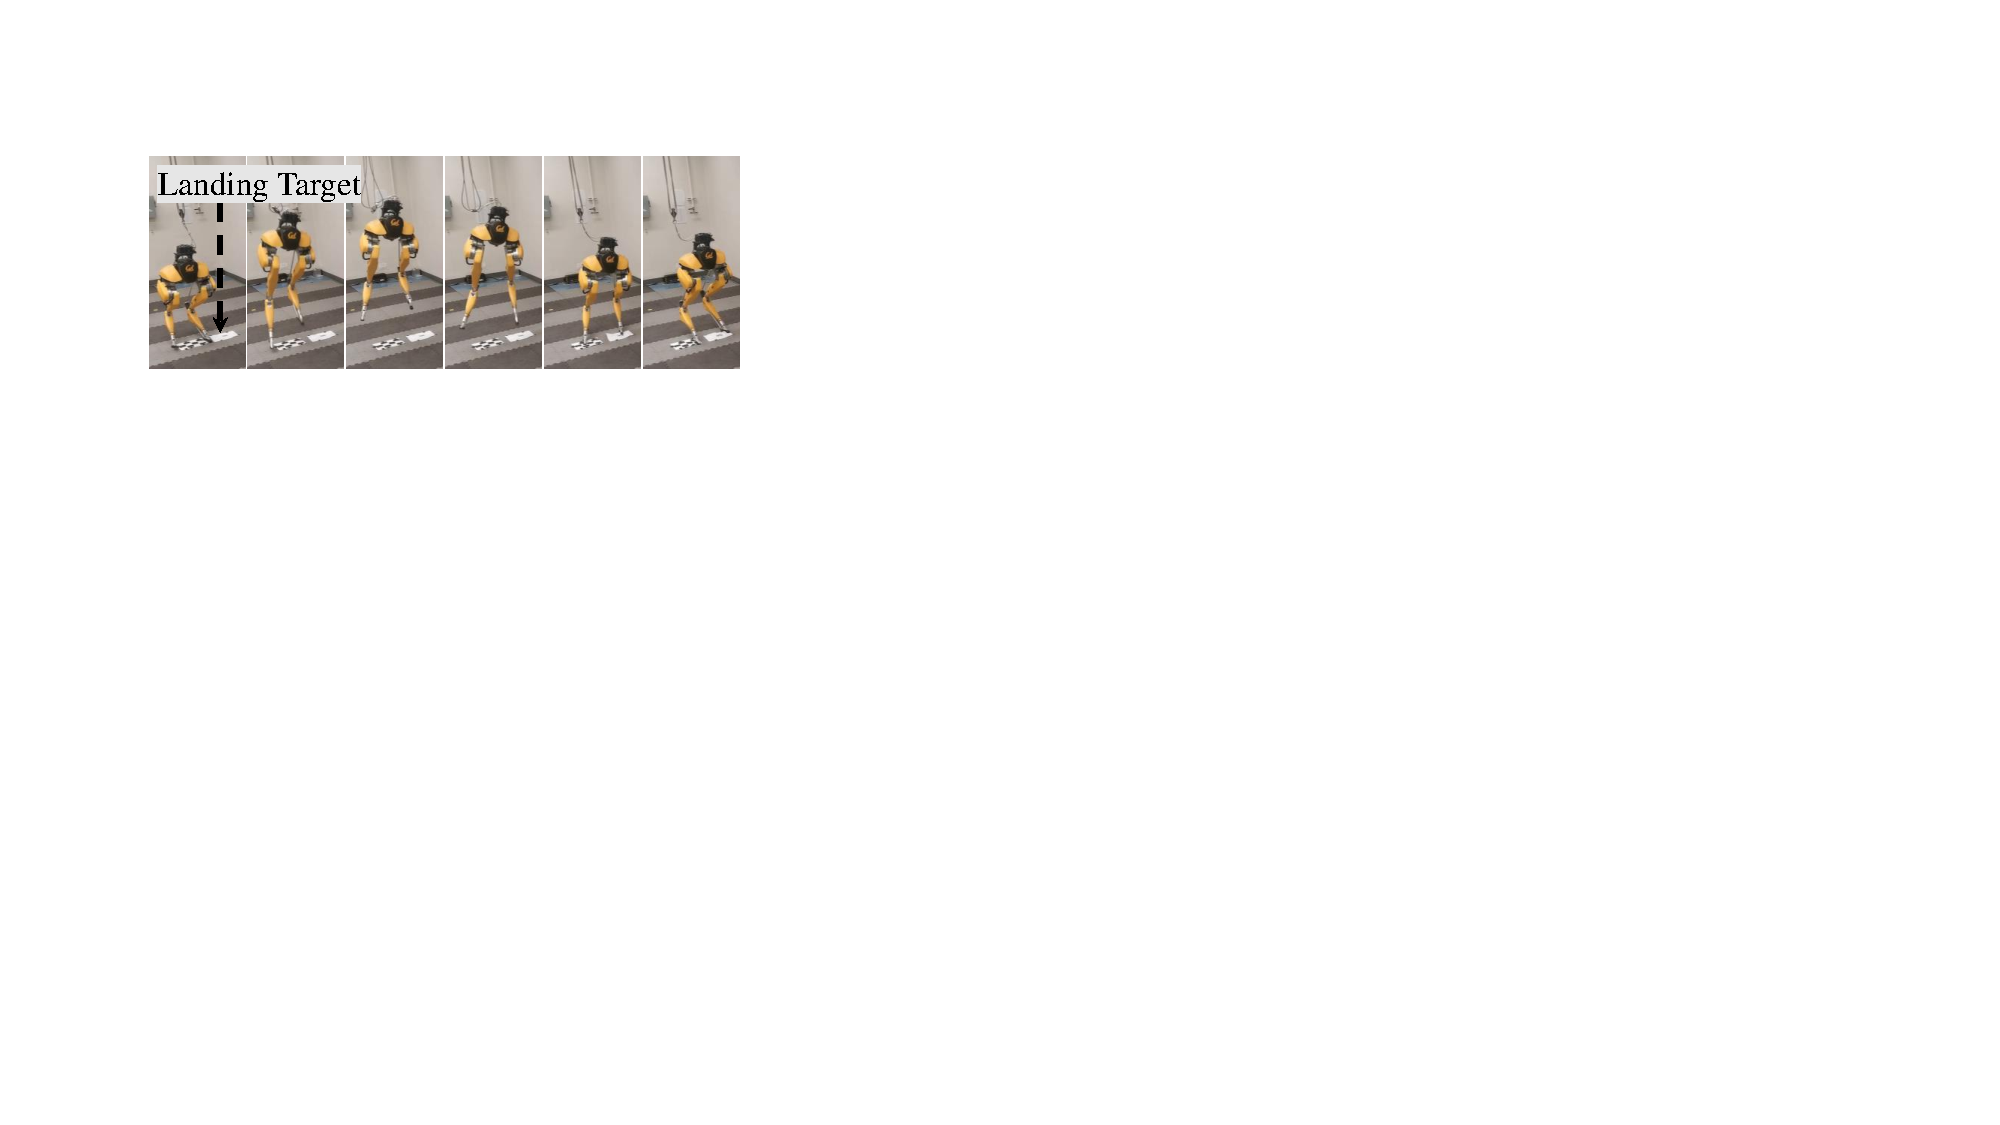
\includegraphics[width=\linewidth]{figures/jump_flat_lateral03_appx.pdf}
  \caption{$(q^d_x, q^d_y, q^d_\phi)$ = (0m, 0.3m, 0$^\circ$)}
  \label{subfig:jump_flat_lateral03_appx}
\end{subfigure}
\begin{subfigure}{0.53\linewidth}
  \centering
  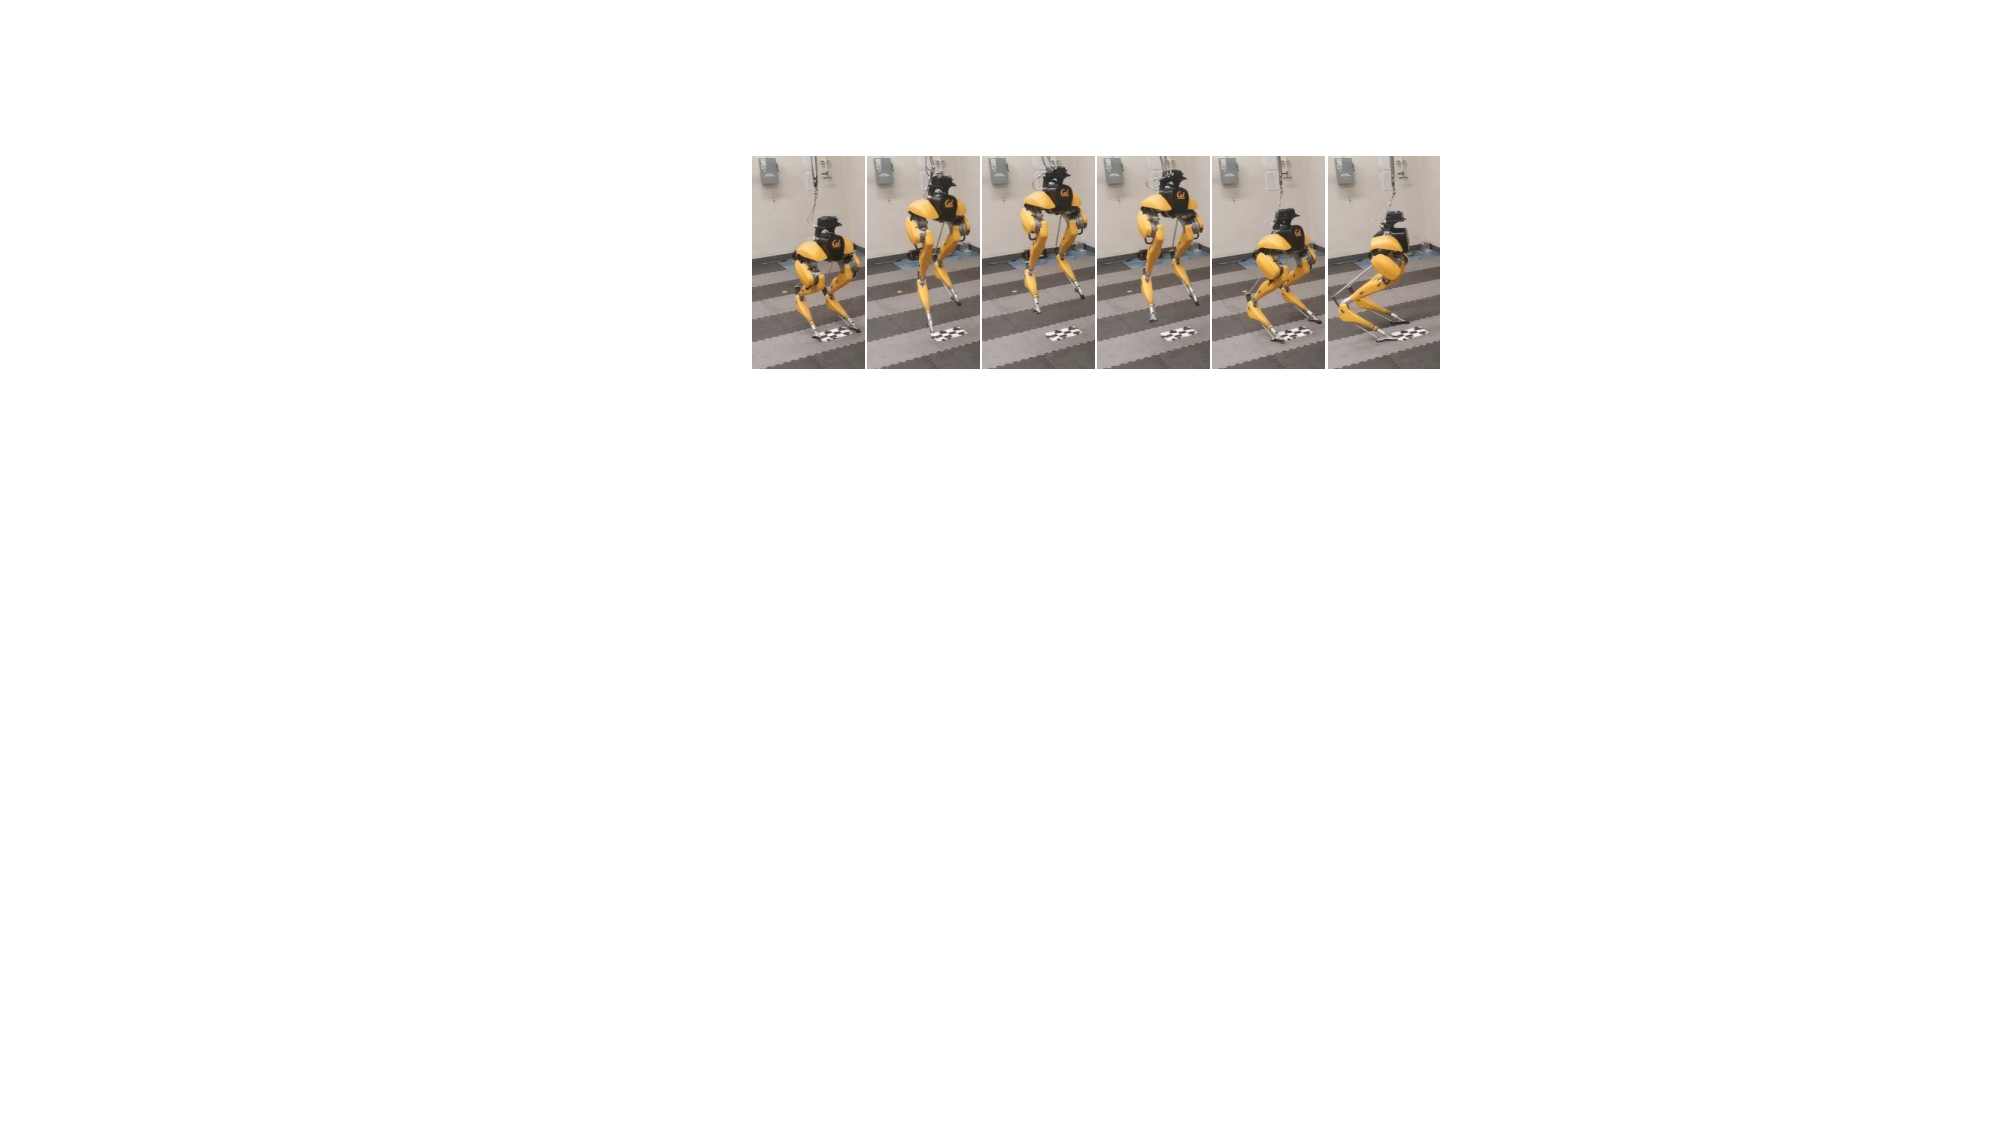
\includegraphics[width=\linewidth]{figures/jump_flat_turn60_appx.pdf}
  \caption{$(q^d_x, q^d_y, q^d_\phi)$ = (0m, 0m, 60$^\circ$)}
  \label{subfig:jump_flat_turn60_appx}
\end{subfigure}
\begin{subfigure}{\linewidth}
  \centering
  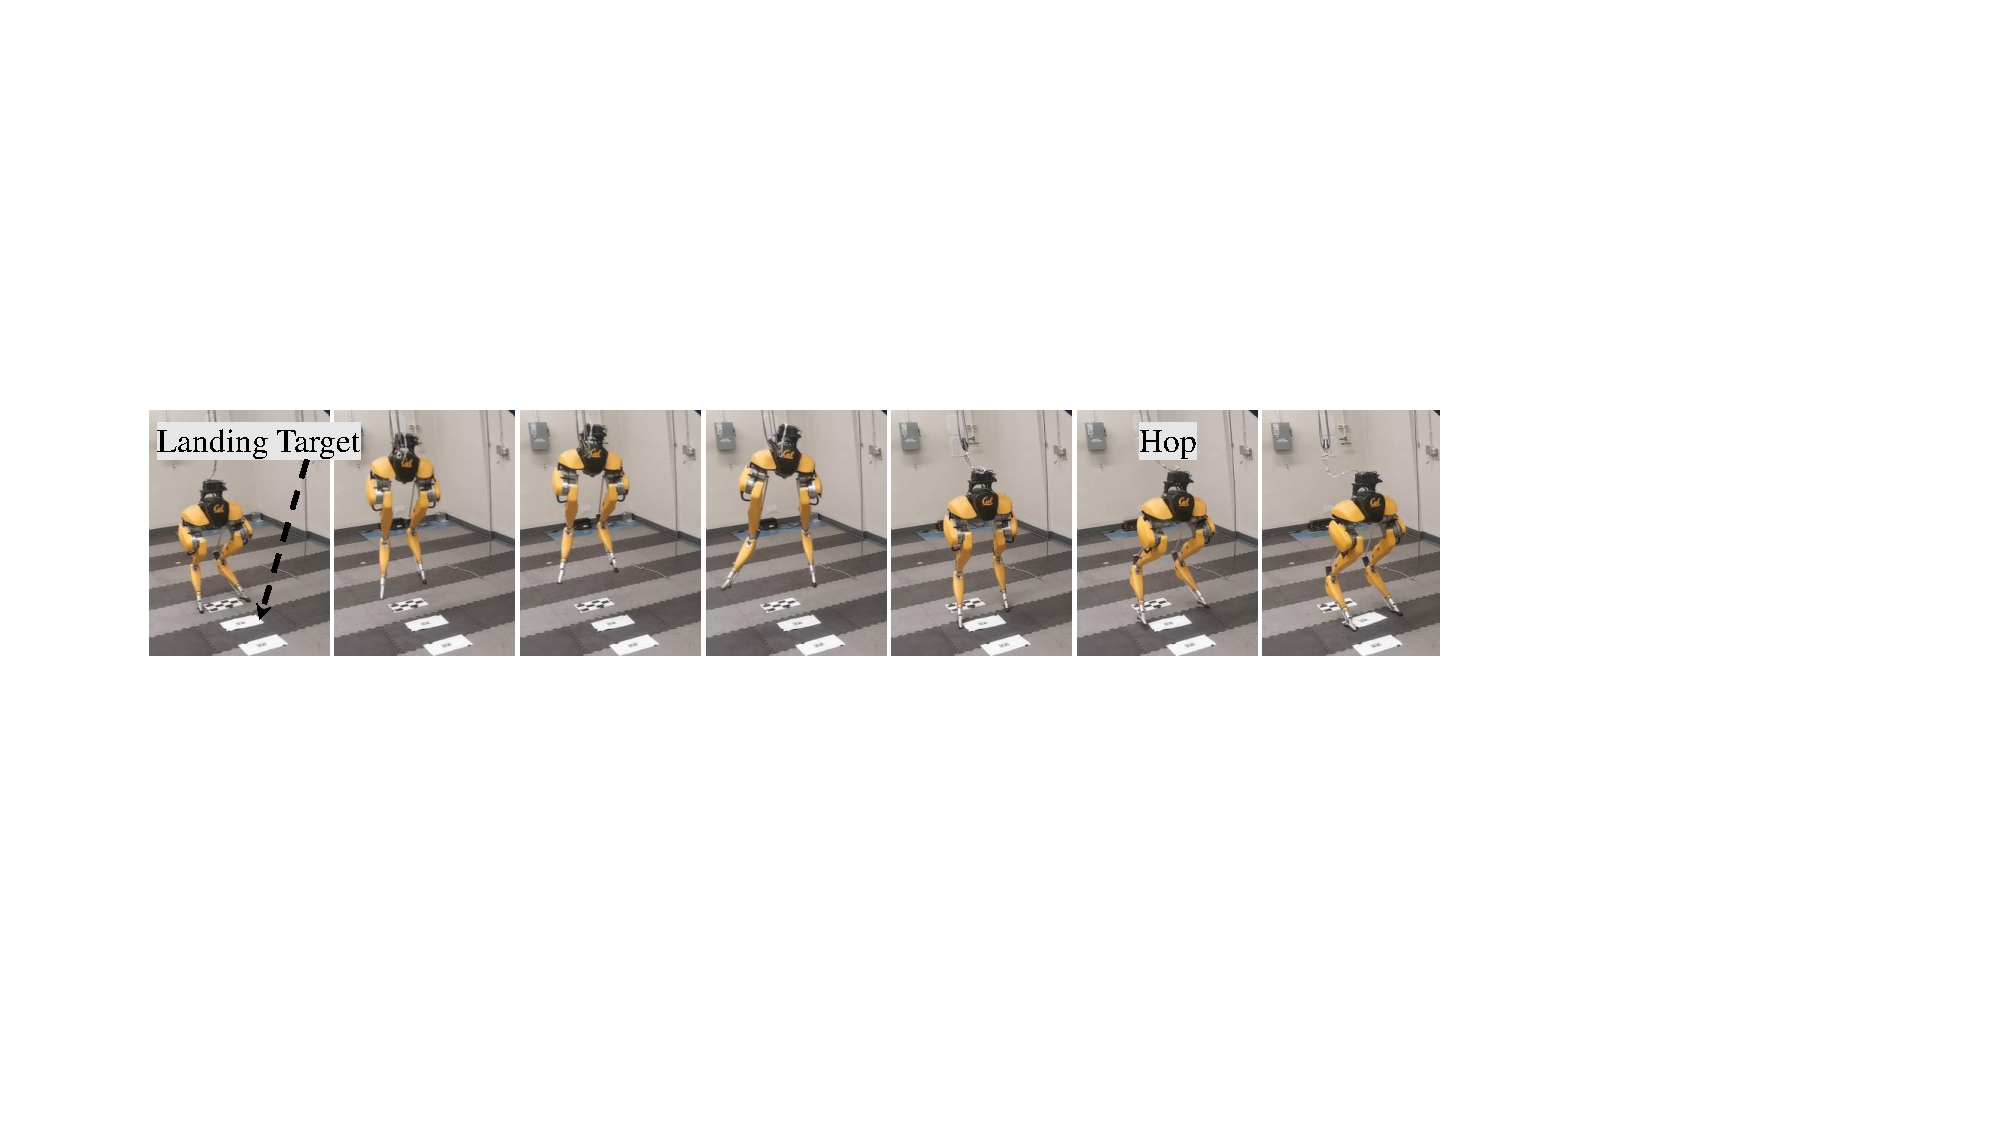
\includegraphics[width=\linewidth]{figures/jump_flat_forward05_appx.pdf}
  \caption{$(q^d_x, q^d_y, q^d_\phi)$ = (0.5m, 0m, 0$^\circ$)}
  \label{subfig:jump_flat_forward05_appx}
\end{subfigure}
\begin{subfigure}{\linewidth}
  \centering
  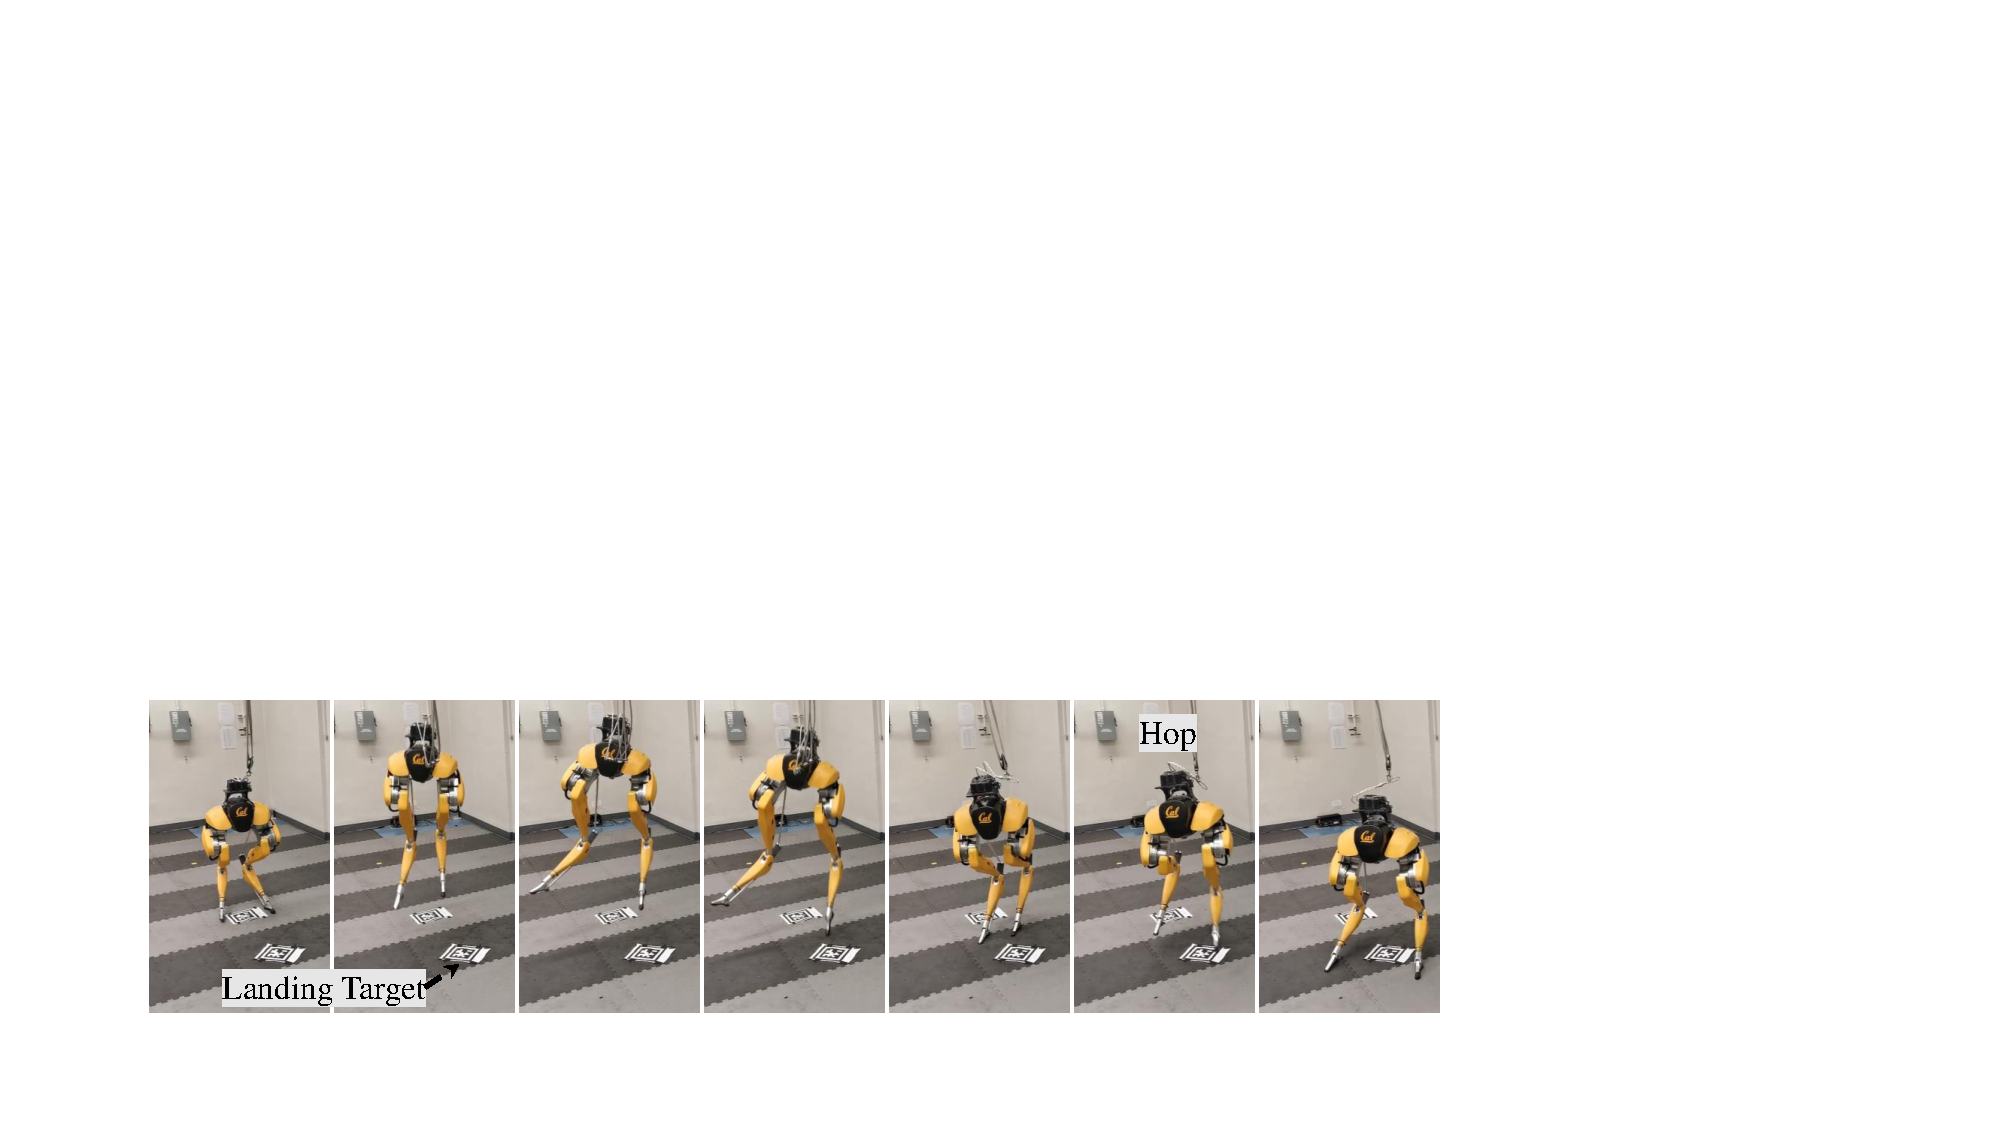
\includegraphics[width=\linewidth]{figures/jump_flat_foward07turn45_appx.pdf}
  \caption{$(q^d_x, q^d_y, q^d_\phi)$ = (0.7m, 0m, -45$^\circ$)}
  \label{subfig:jump_flat_foward07turn45_appx}
\end{subfigure}
\caption{More bipedal jumps using the same flat-ground jumping policy. The paper tag on the ground indicates the jumping target.}\label{fig:more_jumps}
\end{figure}


\subsection{Diverse Bipedal Jumps}~\label{appendix:other_jumps}
Using the same flat-ground jumping policy that realized various bipedal jumps demonstrated in Sec.~\ref{subsec:exp_jumping}, we further evaluate the capacity to jump to other different targets in the real world, as showcased in Fig.~\ref{fig:more_jumps}.


